% document and page typologies
\documentclass[a4paper, onecolumn]{report}

% packages loading
\usepackage[T1]{fontenc}
\usepackage{float}
\usepackage[utf8]{inputenc}
\usepackage[english]{babel}
\usepackage{mathptmx}
\usepackage{geometry}
\usepackage{graphicx}
\graphicspath{ {figures/} }
\usepackage{array}
\usepackage{titlesec}
\usepackage[margin=1pt, font=small]{caption}
\usepackage{subfig}
\usepackage{amsmath}
\usepackage{amsfonts}
\usepackage{mathtools}
\usepackage{amsbsy}
\usepackage{bm}
\usepackage{morefloats}
\usepackage{lettrine}
\usepackage{amsthm}
\usepackage{hyperref}
\usepackage{listing}
\usepackage{enumerate}
\usepackage{algorithm}
\usepackage{caption}
\usepackage{fancyhdr}
\usepackage{listings}
\usepackage{tabularx}
%\usepackage{algorithmic}
\usepackage[noend]{algpseudocode}

\newcolumntype{Y}{>{\centering\arraybackslash}X}

% text style
\geometry{top=2cm, left=3cm, right=3cm, bottom=3cm}

\pagestyle{fancy}
\fancyhf{}
\fancyhead[EL]{\nouppercase\leftmark}
\fancyhead[OR]{\nouppercase\rightmark}
\fancyhead[ER,OL]{\thepage}


\titlespacing{\title}{0pt}{*5}{*0}
\titlespacing{\section}{0pt}{*4}{*0}
\titlespacing{\subsection}{0pt}{*1}{*0}
\titlespacing{\subsubsection}{0pt}{*1}{*0}
\DeclareMathAlphabet{\mathcal}{OMS}{cmsy}{b}{n}
\newcommand{\newln}{\right.  \notag \\ &\left.}
\setlength{\intextsep}{10pt} % Vertical space above & below [h] floats
\setlength{\textfloatsep}{1pt} % Vertical space below (above) [t] ([b]) floats
\setlength{\abovecaptionskip}{10pt}
\setlength{\belowcaptionskip}{10pt}
%\font\largefont=yinitas
%\renewcommand{\labelitemii}{$\bullet$}

\begin{document}
\Large
\sloppy


\tableofcontents
\newpage

\chapter{Introduction}

Within the wide field of robotics, mobile robots gained much attention in recent years, because of the great ambit in which they can be involved in (Figures 1.1, 1.2 and 1.3). Just to mention some of the areas of interest in which mobile robots are requested to operate, consider animation of digital characters, space exploration, mapping of and navigation in unknown and/or changing environments. \\
For accomplishing the greatest part of aforementioned tasks, a robot is often required to plan a path and a series of actions, avoiding obstacles and trying not to hurt itself and the humans potentially at its reach. Path planning and actions can be surely managed via an accurate melting of control theory, mechanics and geometry, but all the process can't disregard an exhaustive knowledge of ambient. That is why mobile robots are equipped with a series of sensors (sonars, cameras, laser scanners, ...) which allow to perceive elements in the surroundings that are useful to derive a reliable structure of environment.
\begin{figure}[htb]
\centering
\centering\setlength{\captionmargin}{0pt}%
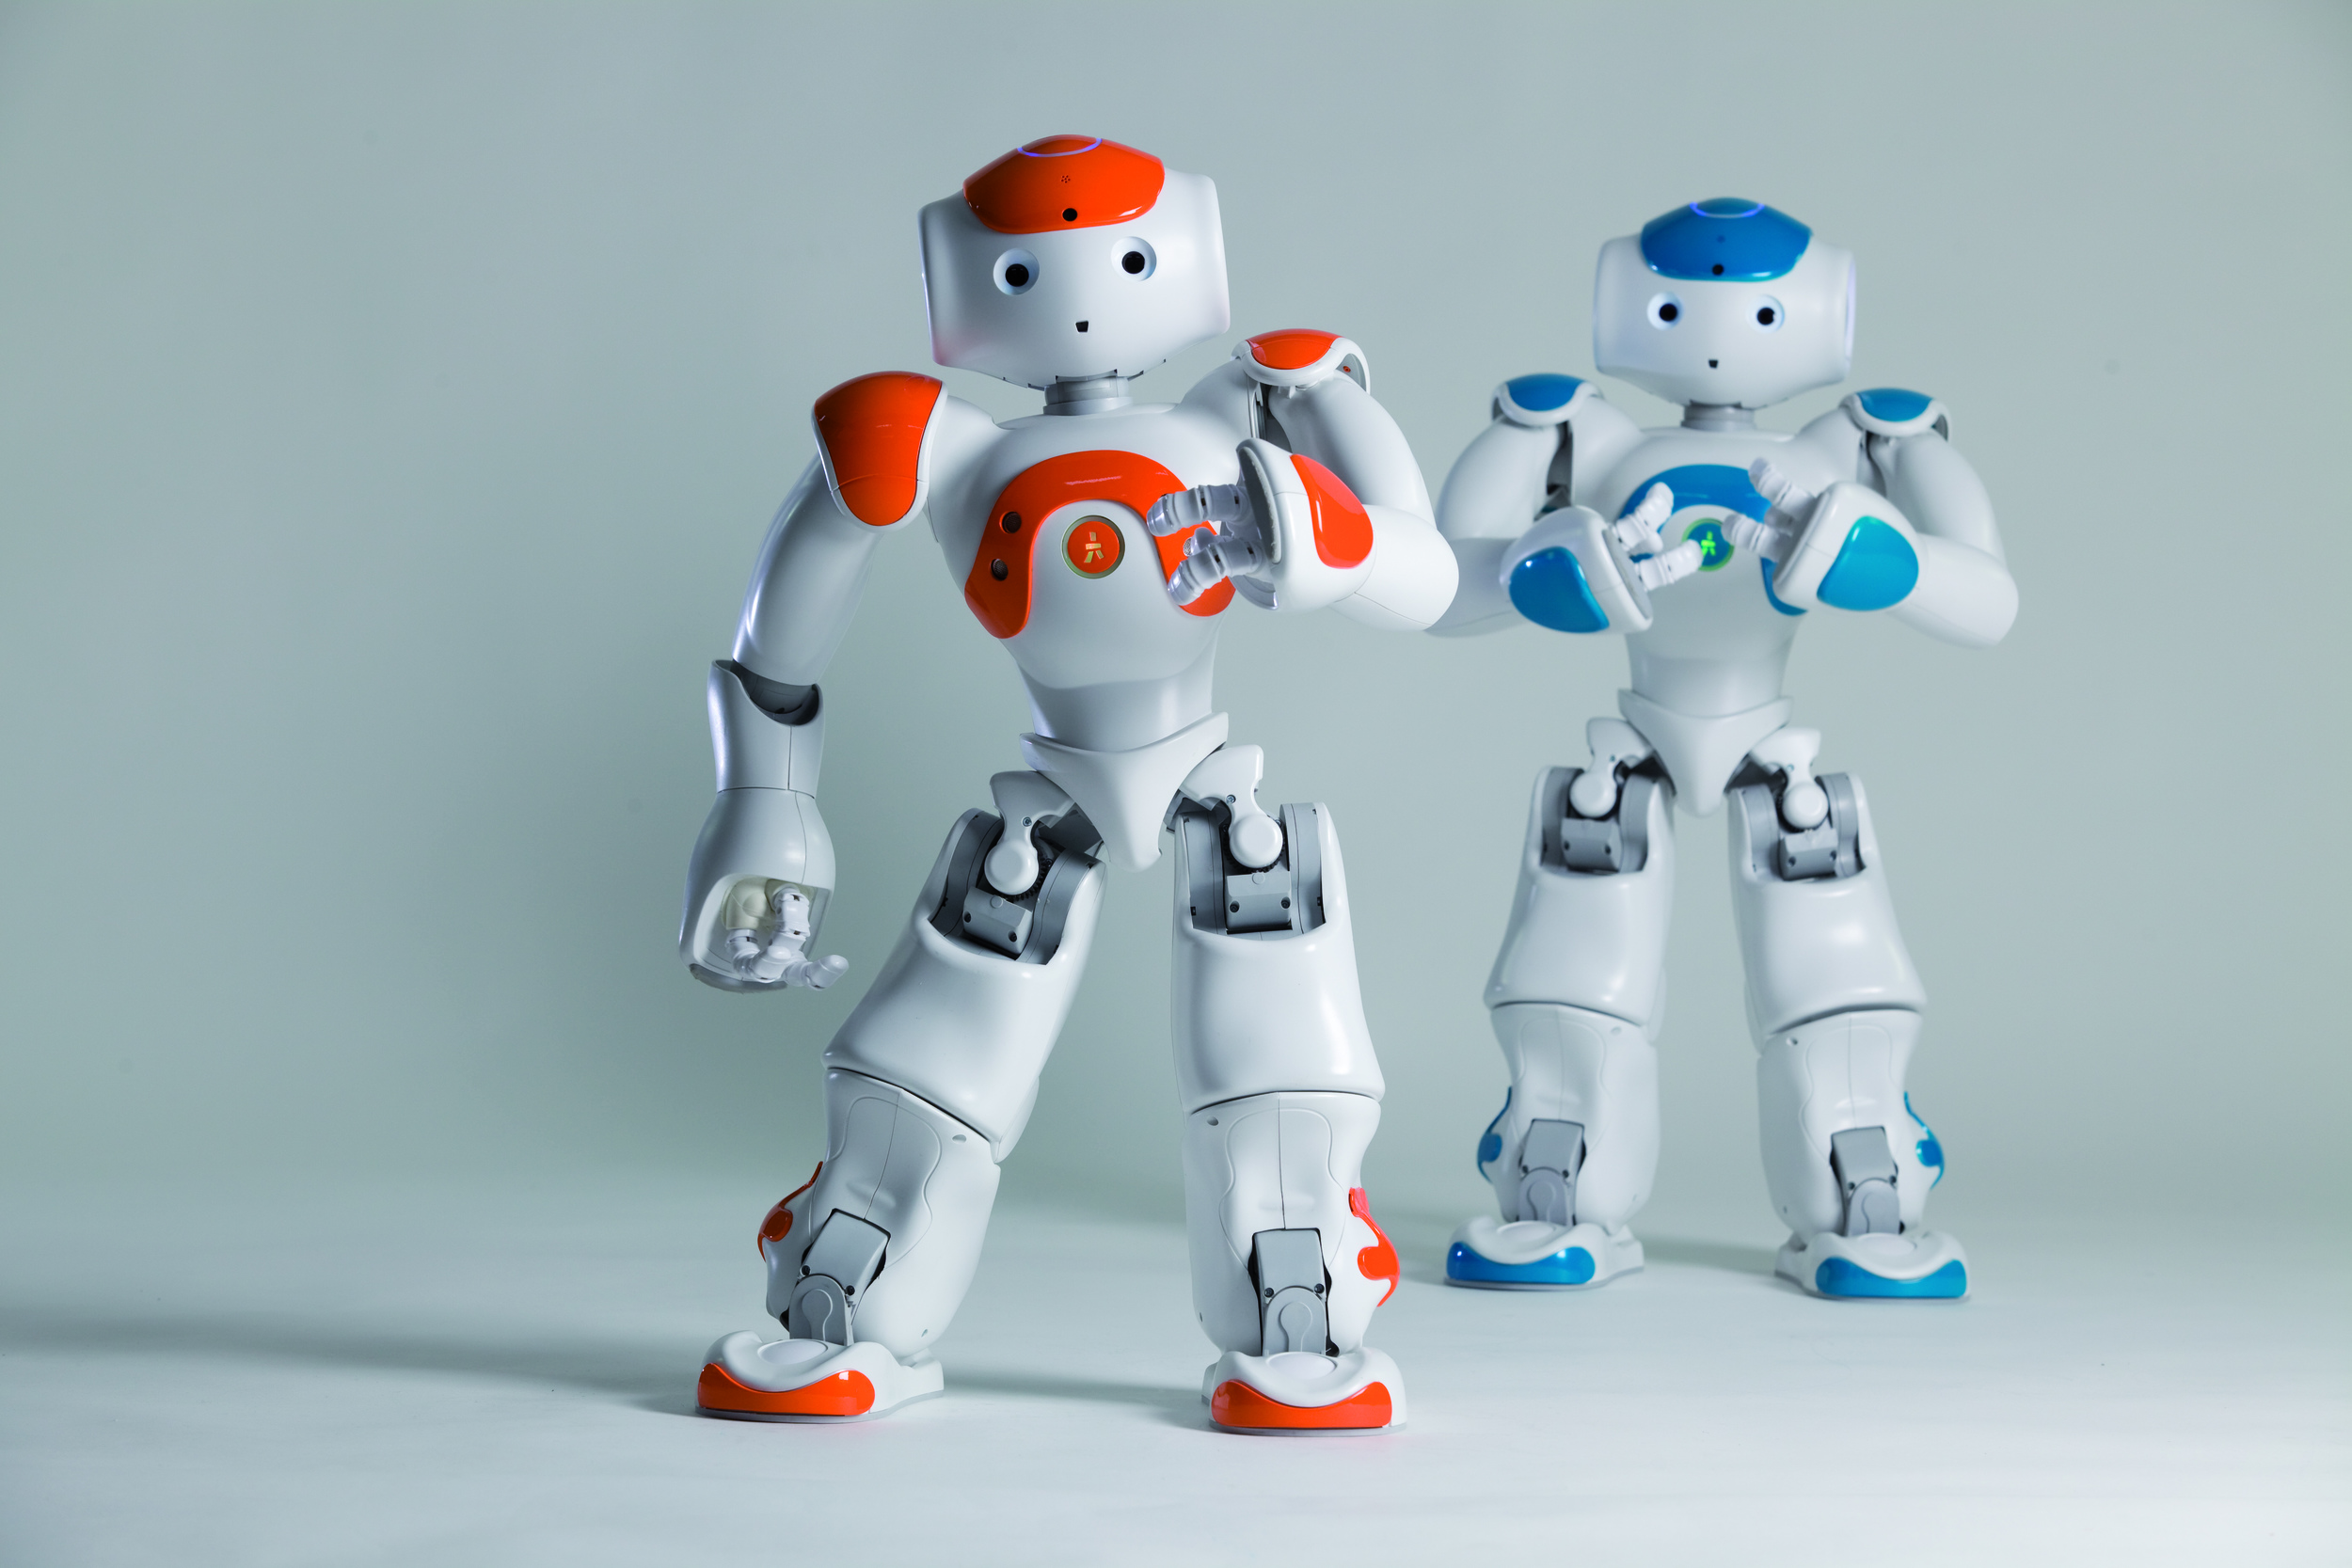
\includegraphics[width=.90\textwidth]{images/nao.jpg}
\caption{The Nao humanoid robot, used for research and reproduction of human behaviour}
\end{figure}

\begin{figure}[htb]
\centering
\centering\setlength{\captionmargin}{0pt}%
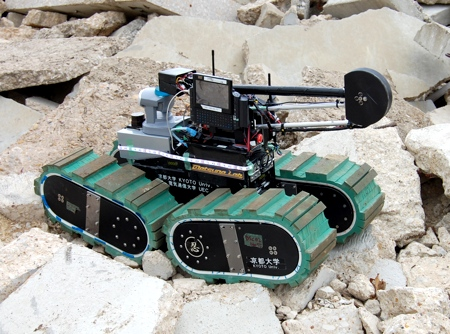
\includegraphics[width=.90\textwidth]{images/rescue.jpg}
\caption{A robot used during rescue operations}
\end{figure}

\begin{figure}[htb]
\centering
\centering\setlength{\captionmargin}{0pt}%
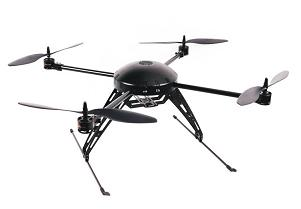
\includegraphics[width=.90\textwidth]{images/quadrotor.jpg}
\caption{A quadrotor, used for aerial video shootings and observation of endangered areas}
\end{figure}

Learning the structure of ambient is not the only result that can be obtained by analysing measurements returned by sensors; indeed, such data, can be exploited to reconstruct the set of poses assumed by robot (in terms of position in space and orientation) in time, while observing world through its sensors. \\
Tracking a robot along its path is a building block of many modern robotics applications, such as \emph{localisation} (which allows a robot to estimate its own position inside an ambient) and \emph{simultaneous localisation and mappig} or \emph{SLAM}, the process of constructing a map of ambient in which a self-localisation procedure is executed.

A lot of research has been done in last decades to perform robot tracking and environment mapping in the attempt to gather the maximum information from sensors. \\
A good example is \emph{visual odometry}, used to determine the position and orientation of a robot through the data returned by a camera. Visual odometry solves the problem of impossibility to apply standard odometry algorithms to mobile robots that have no wheels and no encoders, consequently. Classical odometry, moreover, suffers measurement errors due to wheels' slippages and sliding; such errors, accumulate over time and cause odometry readings to be unreliable. A visual approach, on the other hand, allows to bypass the classical odometry's issues by exploiting the sequential camera images to estimate travelled distance. This requires to determine the \emph{optical flow} field, describing the apparent displacement of objects, caused by relative motion between an observer (a camera or human eye) and an observed scene (Figure 1.4). \\
Another class of algorithms that took advantage from research in the fields of robot tracking and environment mapping is known as \emph{visual SLAM (VSLAM)}; the main goal of algorithms belonging to such class is building a sparse or dense 3D model of a scene while traversing it, determining, at the same time, the trajectory of robot, exploiting a camera and/or other kinds of sensors. 

Visual odometry and VSLAM, along with a long series of other algorithms, base their operations on determining and extracting interesting elements, known as \emph{features}, from subsequent sensor readings and trying to track their position across such acquisitions. Regarding the features to be extracted, there is not a unique choice, since performance requirements have a crucial role in determining a good selection; usually, lines or points with particular properties (for example, the ones returned by the well known \emph{scale-invariant feature transform} or \emph{SIFT}) represent a nice option.
The features matching permits to find the rigid transformation that best aligns two laser scans or camera frames, solving the so called \emph{scan matching} problem. \\
The approach to the research of desired transformation is not unique, as one may imagine; a possible resolution can be achieved using a probabilistic formulation of the problem, for instance maximising the quantity $p(x_t|x_{t-1}, u_t, y_t, y_{t-1})$, expressing the probability to have, at the time $t$, the robot pose $x_t$, given the previous pose $x_{t-1}$, the current and previous sensor readings $y_t$ and $y_{t-1}$, the current odometry measurements $u_t$. \\
An alternative formulation can be obtained for point features if an initial set of association is known; in this case, minimising a squared error function, it is possible to retrieve sought transformation in closed form. When initial set of correspondences is not available at the beginning, it can be constructed using a random sampling of points or using a data association policy (for example, coupling each point to its nearest neighbour).\\
\begin{figure}[htb]
\centering
\centering\setlength{\captionmargin}{0pt}%
\vspace*{0.06in}
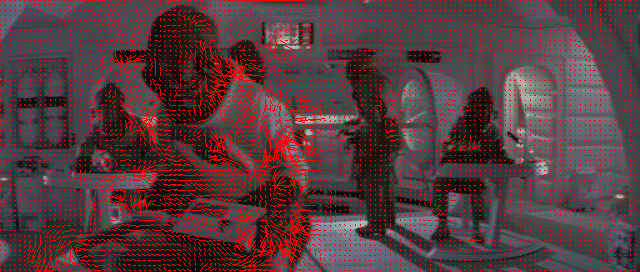
\includegraphics[width=.90\textwidth]{images/optical_flow.png}
\caption{Example of an optical flow: the red arrows indicate how the content of a single pixel moved from its original position, across frames}
\end{figure}
In this thesis we will introduce a new method to solve scan matching issue, presenting it, in an innovative fashion, as a least square estimation problem. The performances of the algorithm we will present will show that chosen approach reveals to be very fast and effective, as confirmed by the convergence analysis reported in last chapter. Moreover, after testing on real data, we will determine that presented algorithm compares favourably with state of the art approaches in contexts for which it was designed.

The outline of thesis can be summarised in the following list:
\begin{itemize}
	\item{\emph{Chapter 2} shows some state of the art approaches for the resolution of problems regarding scan matching and features selection}
	\item{\emph{Chapter 3} introduces the basic concepts on which thesis is based, such as sensors, odometry and feature extraction. The theory at the basis of implemented least square approach is presented}
	\item{\emph{Chapter 4} exposes the algorithm for scan matching resolution, by explaining each of its parts and how all them work together}
	\item{\emph{Chapter 5}, finally, shows the results obtained by testing separately the modules composing our algorithm and by testing the system as a whole}
\end{itemize}

\chapter{Related work}
\section{Introduction}
Self localisation of robot inside a unknown environment passes through the extraction of relevant patterns from data acquired by sensors on-board. Such patterns, usually called \emph{features}, must be chosen carefully and tested, in order to realize whether their are suitable for the task to be accomplished. \\
In this chapter, we will describe a procedure to estimate how much a certain features is useful, by exploiting the concept of \emph{dissimilarity}, i.e. a measure of how much a sensor's perception (an image taken by a camera, for instance) changes with respect to a reference one.

The same importance must be given to the way we choose to represent a feature, in order to be able to individuate it when it figures out in different scans of robot. In this thesis, we decided to use lines as features; we will describe, then, in the beginning of this chapter, how the polar representation of a line was exploited in Hough domain, to individuate an algorithm able to solve the so called \emph{scan matching} problem. \\ 
We will introduce, moreover, an other procedure that takes advantage of the geometric structure of environment and updates a list of plausible matches between lines in different scans. The output of procedure is melted with data from odometry, in order to update current robot's pose, through the use of Kalman filters.

\section{Related work in scan matching}
Given two sets of 2D data, the \emph{scan matching} problem consists in finding a translation $T$ and a rotation $R_\phi$ that maximize the overlapping between the two sets. The scan matching algorithms usually work using data furnished by 2D range sensors and differ in their behaviour depending on the availability of an initial guess of solution. \\
A further classification of scan matching algorithms can be made on the basis of their assumption about the presence of noise in sensor's measurements and of features in surrounding environment. Feature-based algorithms, in particular, gained a great success because of their computational effectiveness, but it must be underlined that the extraction of features may produce a loss of information. 

When ambient contains features that are invariant to rotation and translation, they can be easily extracted from scans and can be used to find a solution in a linear time. \\
If the extraction of features is not simple because of the structure of environment, then it is possible to use algorithms belonging to ICP family, which base their operation on a two step procedure:
\begin{itemize}
	\item{find an initial heuristic set of correspondences between points in two scans}
	\item{find a roto-traslation that more or less satisfies the set of correspondences}
\end{itemize}
The two steps are repeated until the error falls below a certain threshold. The convergence is possible if scans are produced in two robot's positions that are close to each other.

\subsection{Scan matching using the Hough transform}
In a 2009 article by Censi, Iocchi and Grisetti, the problem of scan matching is afforded by the use of \emph{Hough transform (HT)} and is, then, moved to the Hough domain. If we have an \emph{input space} $\mathcal{S}$, the HT maps an input $i(\bf{s})$ (with $\bf{s} \in \mathcal{S}$) to an output function $\mbox{HT}\{i\}(\bf{p})$, with $\bf{p}$ belonging to a \emph{parameter space} $\mathcal{P}$. \\
We can define the HT of input $i(\bf{s})$ as
\begin{equation}
	\mbox{HT}[\mathcal{F}, i](\bf{p}) = \int_{\mathcal{F}_{\bf{p}}} \emph{i}(\bf{s}) \emph{d}\bf{s}
\end{equation}
A possible choice for $\mathcal{P}$ is the the set of representations of lines in $\mathbb{R}^2$. If we recall the polar representation of lines 
\begin{equation}
	x\cos\theta + y\sin\theta = \rho
\end{equation}
in which $\theta$ expresses the direction of line's normal vectors and $\rho$ its distance from origin (see Figure 1.1), we can select a family of sets to apply HT:
\begin{equation}
	\mathcal{F}_{(\theta, \rho)} =\{(x,y) | x\cos\theta + \sin\theta = \rho\}
\end{equation}
On the other side, the input space is composed by points $P = \{p_j\}$, as they are returned by a range sensor. So we have that
\begin{equation}
	\bf{s} := \emph{(x,y)} \in \mathcal{S} := \mathbb{R}^\emph{2}
\end{equation}
and
\begin{equation}
	i(\bf{s}) = \sum_{\emph{j}} \delta(\bf{s} - \bf{p_j})
\end{equation}
where $\delta$ is Dirac's impulse distribution.

HT has two fundamental properties:
\begin{itemize}
	\item{\mbox{HT}$(\theta, \rho)$ is 2$\pi$-periodic}
	\item{the two points $(\theta, \rho)$ and $(\theta+\pi, -\rho)$ in $\mathcal{P}$ represent the same line in $\mathbb{R}^2$}
\end{itemize}
Let's suppose that $\emph{i}(\bf{s})$ and $\emph{i'}(\bf{s})$ are two inputs, such that
\begin{equation}
	\emph{i'}(\bf{s}) = \emph{i}(\emph{R}_\phi \cdot \bf{s} + \emph{T})
\end{equation}
Then, within parameter space $\mathcal{P}$:
\begin{equation}
	\mbox{HT}'(\rho, \theta) = \mbox{HT}(\theta+\phi, \rho+(\cos\theta \quad \sin\theta)T)
\end{equation}
Computing the HT passes through a discrete approximation of it, called \emph{Discrete Hough Transform (DHT)}; the comparison with simple HT is shown in Figure 1.2. DHT allows to redefine our family of sets as:
\begin{equation}
	\mathcal{D}_{(\theta, \rho)} = \{(x,y) | \ \rho\le x\cos\theta + y\sin\theta < \rho + \Delta\rho\} 
\end{equation}
\begin{figure}[htbp]
\centering
\begin{minipage}[c]{.40\textwidth}
\centering\setlength{\captionmargin}{0pt}%
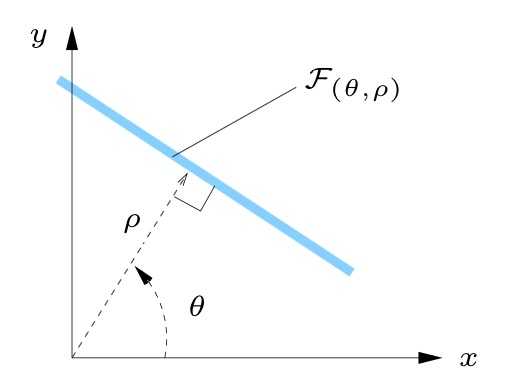
\includegraphics[width=.90\textwidth]{images/ht.jpeg}
\caption{Hough transform}
\end{minipage}%
\hspace{10mm}%
\begin{minipage}[c]{.40\textwidth}
\centering\setlength{\captionmargin}{0pt}%
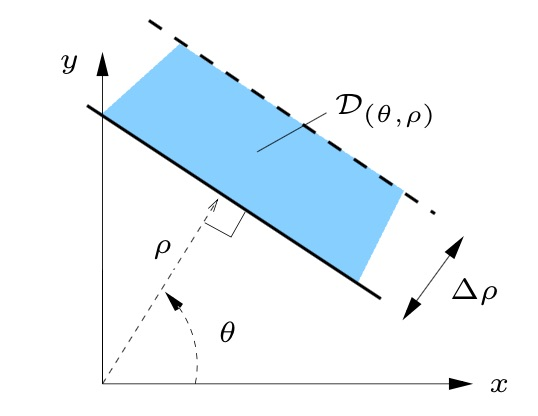
\includegraphics[width=.90\textwidth]{images/dht.jpeg}
\caption{Discrete Hough transform}
\end{minipage}
%\caption{Didascalia comune alledue figure\label{fig:minipage2}}
\end{figure}
For a complete definition of the scan matching algorithm based on HT, we need to define the so called \emph{Hough spectrum}. For such purpose, we need a funcional $g$ that is invariant to traslation. Theoretically speaking, this means that, given a function $f$:
\begin{equation}
	f'(\tau) = f(\tau + \alpha) \Rightarrow g[f] = g[f']
\end{equation}
So, it is possible to define the Hough Spectrum as
\begin{equation}
	\mbox{HS}_g[i](\theta) := g[\mbox{HT}[i](\theta, \cdot)]
\end{equation}
An interesting property of spectrum is its \emph{invariance}. If we define again two inputs $i(\bf{s})$ and $i'(\bf{s})$ as in (), the following statement is valid:
\begin{equation}
	\mbox{HS}_a[i](\theta) = \mbox{HS}_a[i'](\theta + \phi).
\end{equation}
This property, in case of the use of DHT in place of HT, holds only if the quantity $(\cos \theta \quad \sin \theta)T$ is a multiple of $\Delta\rho$.

The set of possible choices for $g$ is wide and a natural one is the energy of the sequence in discrete domain:
\begin{equation}
	g[f] = \sum_i f_i^2
\end{equation}
Since the property illustrated in () holds, it is possible to estimate $\phi$ by correlating the discrete spectra of sensor data $\mbox{DHS}^S(\theta)$ and of reference data $\mbox{DHS}^R(\theta)$. Then, local maxima of correlation are ordered; beginning with the greatest maximum, proceeding up to a chosen number, a new hypothesis for $\phi$ is formulated. \\
We can suppose that, if $\Phi$ is the domain in which we search for the value of $\phi$, such domain can have an upper and lower bound, in such a way that $\Phi = [-\phi_U, \phi_U]$. If this assumption cannot be made, then it can be simply set $\Phi = [-\pi, \pi]$. \\
The correlation between the two spectra can be obtained using the relation
\begin{equation}
	\mbox{corr}_{DHS}(\phi) = \sum_{\theta \in \Theta} \mbox{DHS}^S(\theta) \cdot \mbox{DHS}^R(\theta - \phi)
\end{equation}
The hypotheses ${\phi_1, \dots, \phi_k}$ are retrieved from local maxima of correlation.

The scan matching problem is almost solved; what remains to be done is the estimation of traslation $T$. Let's assume $\phi=0$ (this can be obtained by shifting the columns of $\mbox{DHT}^S$ and $\mbox{DHT}^R$ by the $\phi$ previously computed). We can choose an arbitrary $\theta = \hat{\theta}$. According to (), we can derive that
\begin{equation}
	\mbox{DHT}^R(\hat \theta, \rho) = \mbox{DHT}^S(\hat \theta, \rho + (\cos \hat \theta \quad \sin\hat\theta)T)
\end{equation}
By correlating the columns of $\mbox{DHT}^R$ and $\mbox{DHT}^S$, the projection of $T$ onto the direction $\hat\theta$, $(\cos\hat\theta \quad \sin\hat\theta)T = d(\hat\theta)$, can be retrieved. Similarly to $\phi$,  a bound $[-|T|_U, |T|_U]$ for searching in the domain of $d(\hat\theta)$ can be set.\\
Considering two different values for $\theta$ and the maximum of correlation, a linear system can be built to find T. Different pairs $(\theta_1, \theta_2)$ furnish different results for $T$, that can be used as different hypotheses or combined to obtain an over-constrained system to be solved with least square estimation:
\begin{equation}
	i = 1 \dots n: \quad (\cos\theta_i \quad \sin\theta_i)T = d(\theta_1)
\end{equation}
The elements of set $\{\theta_1,\dots,\theta_n\}$ can be chosen among the maxima of sensor's DHS, i.e. 
\begin{equation}
	\{\theta_1,\dots,\theta_n\} = \mbox{localMaxOf}\{\mbox{DHS}^S(\phi)\}
\end{equation}

Finally, using the concepts described until this moment, it is possible to create a scan matching procedure, whose main steps can be summarized in the following:
\begin{itemize}
	\item{Compute DHT and DHS for reference and sensor data.}
	\item{Use local maxima of spectra cross-correlation to make hypotheses about $\phi$.}
	\item{For each hypothesis produced at previous step, correlate columns of DHT to get linear constraints on $T$.}
	\item{Proceed following one of two possible paths:}
		\begin{itemize}
			\item{combine linear constraints to get multiple hypotheses about $T$ and order solutions on the basis of a likelihood function}
			\item{produce a dense output by accumulating the results of correlation}
		\end{itemize}
\end{itemize}

\subsection{Scan matching in polygonal environments}
Many of the known matching methodologies require a good estimation of robot's initial pose which, when it is close to actual one, allows to limit the search space. The pose estimation and its update exploit a Gaussian model; thus, pose itself is accurately computed and updates can be calculated using Kalman filters. In particular, the extended Kalman filter models robot's pose as a Gaussian distribution $l(t) \sim N(\mu_l,\Sigma_l)$, using $\mu_l = (x,y,\alpha)^T$ as mean value and a $3\times3$ matrix for covariance $\Sigma_L$.\\
When the robot moves a distance $\delta$ and rotates by an angle $\theta$, such motion can be described as $a \sim N((\delta, \theta)^T, \Sigma_a)$ and robot's pose is updated according to the following relations:
\begin{equation}          
	\begin{aligned}              
		\mu_l &:= E(F(l,a)) = \left(\begin{matrix}x+\delta\cos(\alpha) \\ y + \delta\sin(\alpha) \\ \alpha + \delta\end{matrix}\right) \\
		\Sigma_l &:= \nabla F_l\Sigma_l\nabla F_l^T + \nabla F_a\Sigma_a \nabla F_a^T
	\end{aligned}
\end{equation}
where $E$ is the expected value of function $F$ and $\nabla F_l$ and $\nabla F_a$ are its Jacobians with respect to $l$ and $a$.

From scan matching a pose update $s \sim N(\mu_s, \Sigma_s)$ is obtained, so the robot pose can be updated:
\begin{equation}
	\begin{aligned}
		\mu_l &:= (\Sigma_l^{-1} + \Sigma_s^{-1})^{-1} \cdot (\Sigma_l^{'-1}\mu_l + \Sigma_s^{-1}\mu_s) \\
		\Sigma_l &:= (\Sigma_l^{-1} + \Sigma_s^{-1})^{-1}
	\end{aligned}
\end{equation}

Anyway, the success of Kalman filtering depends mainly on how the scan matching algorithm can estimate robot's pose. That is why, Gutmann, Weigel and Nebel, in 1999, proposed a new scan matching algorithm that exploits the polygonal structure of environment. \\
The procedure, known as \emph{LineMatch}, is described by Algorithm 1.
\begin{algorithm}
	\caption{\mbox{LINEMATCH} (M, S, P)}
	\begin{algorithmic}[1]
		\item{$\bf{Input:} $ model lines M, scan lines S, pairs P}
		\item{$\bf{Output:} $ set of position hypotheses H}
		\item{$\bf{if}$ |P| = |S| $\bf{then}$}
		\item{$\quad$ H := P}
		\item{$\bf{else}$}
		\item{$\quad$ H := $\emptyset$}
		\item{\emph{$\quad$ s := SelectScanline(S, P)}}
		\item{$\quad$\bf{for all} $m \in M$ $\bf{do}$}
		\item{\qquad $\bf{if}$ \emph{VerifyMatch(M, S, P $\cup$ \{(m, s)\}) \bf{then}}}
		\item{\quad \qquad \emph{H := H $\cup$ \{\mbox{LINEMATCH}(M, S, P   $\cup$\{(m, s)\})\}}}
		\item{$\bf{return}$ H}	
	\end{algorithmic}
\end{algorithm}
The main tasks performed by algorithm are extracting lines from current scan and comparing them with the ones contained in a \emph{a priori} map. In particular, function \emph{SelectScanline} picks a a new line to be matched, while \emph{VerifyMatch} checks that a new pair \emph{(m, s)} of matched lines is compatible with the pairs alreary accepted in previous iterations of procedure. Finally, the algorithm returns a set of accepted pairs, that can be translated into positions from which robot may have taken scans (Figure 1.3). Proper constraints on lines' lengths and roto-traslations can allow algorithm to be more effective; this implies that it is not necessary to have a good estimate of robot's initial pose, since robot is able to recover from initial error.  
\begin{figure}[htbp]
\centering
\centering\setlength{\captionmargin}{0pt}%
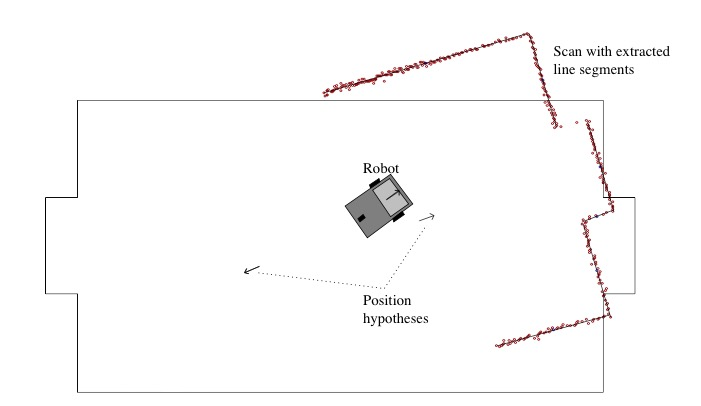
\includegraphics[width=.90\textwidth]{images/robocup_robot_positions.jpeg}
\caption{Example of two possible position hypotheses returned by LINEMATCH}
\end{figure}
Once the matching activities are completed, the most plausible position is selected using odometry (a closest neighborhood policy will fit for the purpose) and is used to update robot's pose, by Kalman filters. A good choice for initial mean and covariance values may be 
\begin{equation}
	\begin{aligned}
		\mu_l &:= \left(\begin{matrix}0 & 0 & 0\end{matrix}\right)^T \\
		\Sigma_l &:= \left(\begin{matrix} \infty & 0 & 0 \\ 0 & \infty & 0 \\ 0 & 0 & \infty\end{matrix}\right)
	\end{aligned}
\end{equation}

A summary of full algorithm is shown in Figure 1.4. The modular formulation supposes the presence of an \emph{a priori} knowledge of the field in which robot is requested to operate.
\begin{figure}[htbp]
\centering
\centering\setlength{\captionmargin}{0pt}%
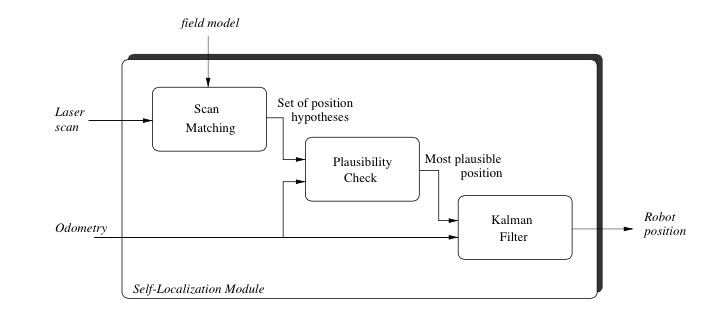
\includegraphics[width=.90\textwidth]{images/robocup_alg_module.jpeg}
\caption{Modular representation of full algorithm}
\end{figure}

\section{Selecting features to track}
A scan matching algorithm, whatever its inner functionalities, can work properly only if the choice of features to extract has been made correctly, in order to maximize matching result. \\
Shi and Tomasi introduced, in 1994, a method for features selection based on the concept of \emph{dissimilarity}, a measure of changes occurred to features between first frame and current one. When dissimilarity is too high, features should be ignored. 

Considering frames acquired by a moving camera, all patterns that can be extracted vary in terms of intensity. Such changes are included in the definition of \emph{motion}:
\begin{equation}
	I(x, y, t+\tau) = I(x-\xi(x,y,t,\tau), y - \eta(x,y,t,\tau)).
\end{equation}
What previous equation states is that an image taken at the instant of time $t+\tau$ can be obtained from one taken at time $t$ by applying a motion, whose entity $\delta = (\xi, \eta)$ is called \emph{displacement} of point $\boldsymbol{x}\emph{= (x, y)}$.

If we speak in terms of windows, we can define the \emph{affine motion field} as 
\begin{equation}
	\delta = D\boldsymbol{x} + d
\end{equation}
with
\begin{equation}
	D = \left(\begin{matrix}d_{xx} & d_{xy} \\ d_{yx} & d_{yy}\end{matrix}\right)
\end{equation}
a deformation matrix; $\boldsymbol{d}$ is the translation of a feature window's center. \\ 
By measuring the coordinates $\boldsymbol{x}$ with respect to the center of window, we get that a point $\boldsymbol{x}$ in the first image $I$ moves to a point $A\boldsymbol{x} + d$ in second image $J$, with $A=\boldsymbol{1} + \emph{D}$ and $\boldsymbol{1}$ a $2 \times 2$ identity matrix. \\
Thus, the tracking problem between two images $I$ and $J$ can be formulated in terms of finding the six parameters contained in $D$ and $\boldsymbol{d}$. A model that uses small windows is preferable, since it causes less problems in terms of depth discontinuity; in such condition, the matrix $D$, that is harder to estimate because of the small variation of motion, can be assumed equal to zero, so
\begin{equation}
	\delta = \boldsymbol{d}. \notag
\end{equation}

The equation () is not satisfied completely, then finding the six unknown motion parameters means to find $A$ and $\boldsymbol{d}$ that minimize dissimilarity
\begin{equation}
	\epsilon = \int \int_W [J(A\boldsymbol{x} + \boldsymbol{d} - I(\boldsymbol{x})]^2 w(\boldsymbol{x})d\boldsymbol{x}
\end{equation}
with $W$ the feature window and $w(\boldsymbol{x})$ a weighting function (in the simpleste case, it can be set to 1. In the other cases, it can be a Gaussian-like function).

When we have a simple traslation, matrix $A$ must coincide with identity matrix. To minimize the value in equation (), it is possible to diffirentiate with respect to unknown parameters in $D$ and $\boldsymbol{d}$ and then set result to zero. The obtained system can linearized by a truncation in Taylor expansion:
\begin{equation}
	J(A\boldsymbol{x} + \boldsymbol{d}) = J(\boldsymbol{x}) + g^T(\boldsymbol{u}).
\end{equation}
This leads to a $6\times6$ system:
\begin{equation}
	T\boldsymbol{z} = \boldsymbol{a}
\end{equation}
with
\begin{equation}
	\boldsymbol{z}^T = \begin{matrix}[d_{xx} & d_{yx} & d_{xy} & d_{yy} & d_x & d_y] \end{matrix}\notag
\end{equation}
The system is completed by an error vector 
\begin{equation}
	\boldsymbol{a} = \int \int_W [I(\boldsymbol{x}) - J(\boldsymbol{x})] \left[\begin{matrix} xg_x \\ xg_y \\ yg_x \\ yg_y \\ g_x \\ g_y  \end{matrix}\right] w \,\, d\boldsymbol{x}
\end{equation}
and a $6\times6$ matrix
\begin{equation}
	T = \int \int_W \left[\begin{matrix}U & V \\ V^T & Z\end{matrix}\right] w \,\, d\boldsymbol{x}
\end{equation}
with 
\begin{equation}
	\begin{aligned}
		U &= \left[\begin{matrix}x^2g_x^2 & x^2g_xg_y & xyg_x^2 & xyg_xg_y \\ x^2g_xg_y & x^2g_y^2 & xyg_xg_y & xyg_y^2 \\ xyg_x^2 & xyg_xg_y & y^2g_x^2 & y^2g_xg_y \\ xyg_xg_y & xyg_y^2 & y^2g_xg_y & y^2g_y^2 \end{matrix}\right] \\ \\
		V^T &= \left[\begin{matrix}xg_x^2 & xg_xg_y & yg_x^2 & yg_xg_y \\ xg_xg_y & xg_y^2 & yg_xg_y & yg_y^2 \end{matrix}\right] \\ \\
		Z &= \left[\begin{matrix}g_x^2 & g_xg_y \\ g_xg_y & g_y^2\end{matrix}\right]
	\end{aligned}
\end{equation}

To be sure to have a good tracking, it is necessary to have a small motion between adjacent frames; this causes $D$ to be small, too, so it can be set to zero. In this situation, determining deformation parameters can be pointless and dangerous as well, since it may lead to solutions with tiny displacements. Indeed, $D$ and $\boldsymbol{d}$ are linked to each other through matrix $V$ and an error in $D$ produces an error in $\boldsymbol{d}$, too. \\
Then, when only $\boldsymbol{d}$ needs to be sought, it is sufficient to solve smaller system
\begin{equation}
	Z\boldsymbol{d} = \boldsymbol{e}
\end{equation}
with $\boldsymbol{e}$ containing the last two elements in $\boldsymbol{a}$. \\
When the two frames to be compared are the first and current ones, a simple traslation model is not suitable and full system should be solved. 

Considering a certain frame, not all its parts contain motion information and not all features are good for tracking, so a selection policy is necessary. A window can be tracked from frame to frame if the matrix $Z$ is well-conditioned; thus, its eigenvalues must be large and cannot differ by too many orders of magnitude. Two small eigenvalues denote a constant intensity within window; a small and large eigenvalues indicate a unidirectional texture pattern; two large eigenvalues may correspond to corners and other easily trackable features. \\
In a few words, a window is accepted if, given the two eigenvalues $\lambda_1$ and $\lambda_2$ of $Z$ we have 
\begin{equation}
	\mbox{min}(\lambda_1, \lambda_2) > \lambda
\end{equation}
with $\lambda$ a chosen threshold.\\
An example of how textures may be extracted and accepted according to condition (1.30) is depicted in Figure 1.5.
\begin{figure}[htb]
\centering
\begin{minipage}[c]{.40\textwidth}
\centering\setlength{\captionmargin}{0pt}%
\centerline{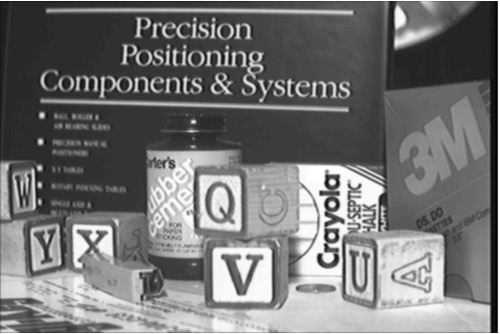
\includegraphics[width=1.5\textwidth]{images/features_original_image.jpeg}}
(a)
\end{minipage} \\
\vspace{10mm}%
\begin{minipage}[c]{.40\textwidth}
\centering\setlength{\captionmargin}{0pt}%
\centerline{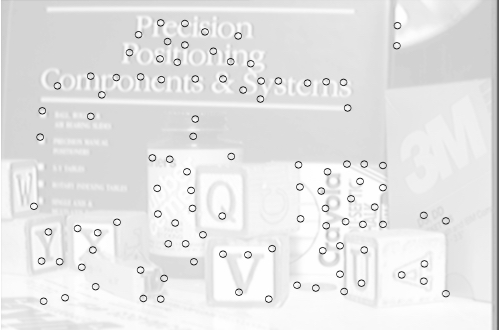
\includegraphics[width=1.5\textwidth]{images/features_extracted_features.jpeg}}
(b)
\end{minipage}
\caption{Original image (a) and extracted features (b), using an acceptance criterion for windows, as explained in 1.30}
\end{figure}
 
%--------------------------------------------------------------------------
\chapter{Basic concepts}
\section{Introduction}
This chapter introduces to the main concepts on which this thesis is based.  \\
First of all, we will concentrate ourselves on describing the concept of sensors and their importance in self-perception of robots. Sensors, indeed, are very useful to allow a robot to localize itself and have an idea of surrounding environment; anyway, to make all this possible, it is necessary to design them in such a way to satisfy a series of requirements. Sensors, although their immense utility, furnish noisy measurements with which localization algorithms must deal.
In this chapter, we will describe one particular kind of sensors, the ones based on the \emph{time of flight (TOF)} method.

The main tecnique used by robots to estimate their current position and orientation is \emph{odometry}, which is based on data returned by robot's encoders. We will analyse the two types of errors it introduces and how they have been experimentally measured.

Data furnished by sensors is often huge, so it is important to extract only relevant parts of it, in order to reduce time in computation. We will describe how such parts can be extracted and which properties we expect them to have.

Finally, we will propose a process based on least squares minimization, that allows to estimate a robot's state (in terms of position and orientation), exploiting the error between measured and expected state value.

\section{Robot sensors}
Robots can be considered, among human artefacts, as the ones closest to the concept of a living being, with their capabilities to sense world and change their own choices on the basis of what they perceive in the surrounding environment. Without a sensing system, robots could be just able to repeat the same task and wouldn't be able to adapt their decisions to an environment continously changing around them. Thanks to sensors, robots can operate in places that are too dangerous for humans and interact with each other. 

When designing a sensor, there is a small set of requirements that should be kept into account:
\begin{itemize}
\item{a good field of view, to satisfy the needings of the greatest number of applications}
\item{a good minimum and maximum range of detection}
\item{the largest accuracy and resolution}
\item{a great ability to detect objects in the environment, dealing with phenomena such as reflection and noise due to ambient interference}
\item{high update frequency, to have real time data at disposal as fast as possible}
\item{generated data should be concise and easy to interpret}
\item{low costs in designing, construction and maintenance}
\item{low power consumption}
\item{small size and weight}
\end{itemize}

\subsection{Range sensors}
In many cases, a robot is required to build a map of its surrounding environment and for such goal a measurement of range between itself and obstacles is needed.
There exists a class of range sensors widely used for such purpose based on the so called \emph{time of flight (TOF)} method; an ultrasonic, RF or optical source generates an energy wave that propagates into ambient and the distance between robot and an object is computed as the product of the velocity of wave and the time required to travel the round-trip distance, according to relation

\begin{equation}
	d = vt
\end{equation}
where $d$ is the round-trip distance, $v$ is the speed of propagation of energy wave and $t$ is the elapsed time. The time interval $t$ in previous equations is the one that elapses while the energy wave reaches the obstacle and gets back to robot; thus, to retrieve the real range between robot and target, $t$ must be divided by two.

The signal emitted by robot reaches an object and walks back on the same way to the robot, where it will be detected by a receiver, that can be located close to emitter or integrated with emitter itself.
As it is evident in ( ), the range to an object can be easily retrieved and no further knowledge about object's nature is necessary.

Similarly to all kinds of sensors, even TOF systems are subject to measurements errors, which can be summarized in the following short list:
\begin{itemize}
\item{\bf{variations in the speed of propagation of emitted signal}}
\item{\textbf{uncertainty in determining when reflected signal was detected}\\ 
Such uncertainties depend on the fact that different surfaces reflect signal differently and this may cause time for detection of returned signal to rise. When a threshold on detection is established, more reflective objects are perceived as closer.}
\item{\textbf{uncertanty in determining the exact round-trip time $t$}\\
 It is due to problems correlated to inner timing circuitry.}
\item{\textbf{interaction between originated signal and surfaces} \\
When source signal hits a surface, only part of it is reflected and perceived by the robot. The remaining part is propagated into ambient or passes through the hit object. Thus, it may happen that no signal is received by robot, particularly if emitting angle exceeds a certain threshold. The part of signal that is not sent back to robot, may be spread to envirnonment and perceived by another robot's sensors.}
\end{itemize}

\section{Odometry}
Odometry is probably the most used method to estimate the position of a robot at any instant in time. The reasons of its success must be found in good accuracy, low cost and high sampling rates. Anyway, the way odometry computes robot's position (by integrating motion information across time) leads to errors; in particular, errors in estimating robot's orientation lead to large position errors, which grow proportionally with the distance afforded by robot. \\
Despite limitations due to errors, odometry gained a great success in mobile robots field, for at the least four reasons:
\begin{itemize}
\item{other kinds of measurements can be itegrated to obtain a better accuracy}
\item{in cases in which landmarks are used for helping to estimate robot's position, their number can be smaller, thanks to odometry's presence}
\item{odometry allows to assume that robot is stuck in a certain pose for enough time to perceive all the landmarks in a given area and compute possible matchings with landmarks detected previously}
\item{in some circumstances, because of the absence of external references (e.g. landmarks) or the impossibility to place any of them in a hostile environment, odometry can be the only way to estimate robot's position}
\end{itemize}
Odometry exploits the measurements obtained from encoders mounted on robot's wheels to extimate its new pose. Let's suppose that, in a certain time interval, robot's wheels have pulses $N_L$ and $N_R$. Let's denote with $c_m$ the conversion factor that allows to convert pulses into a linear displacement. We can suppose that
\begin{equation}
	c_m = \frac{\pi D_n}{nC_e}
\end{equation}
where:
\begin{itemize}
\item{$D_m$ is the nominal wheel's diameter}
\item{$C_e$ is the encoder resolution (pulses per revolution)}
\item{$n$ is the reduction gear ratio between motor and drive wheel}
\end{itemize}
The incremental linear displacements $\Delta U_{L,i}$ and $\Delta U_{R,i}$ for the two wheels can be computed as:
\begin{equation}
	\begin{aligned}
		\Delta U_{L,i} &= c_m N_L \\
		\Delta U_{R,i} &= c_m N_R
	\end{aligned}
\end{equation}

We can now compute the displacement for robot's centerpoint $\Delta U_i$ (that will be taken as a reference for robot's position) and change in orientation $\Delta \theta_i$:
\begin{equation}
	\begin{aligned}
		\Delta U_i &= \frac{\Delta U_R + \Delta U_L}{2}  \\
		\Delta \theta_i &= \frac{\Delta U_R - \Delta U_L}{b}
	\end{aligned}				
\end{equation}
where $b$ is the distance between the two points where wheels touch the ground. 

Thus, the new orientation of robot at time $i$ is:
\begin{equation}
	\theta_i = \theta_{i-1} + \Delta \theta_i
\end{equation}
The new position, at the same instant of time, of its centerpoint will be:
\begin{equation}
	\begin{aligned}
		x_i &= x_{i-1} + \Delta U_i \cos \theta_i \\
		y_i &= y_{i-1} + \Delta U_i \sin \theta_i
	\end{aligned}
\end{equation}

\subsection{Systematic and Non-Systematic errors in odometry}
As explained previously, the odometry exploits three simple equations to estimate current position of robot. All of them, are based on the assumption that any encoder's measurement can be translated into a linear diplacement. Anyway, such assumption may lose its validity in certain circumstances; for instance, if a wheel slips, its encoder will register a measurement that is converted in a linear displacement, even if robot didn't move actually. \\
Slippage is only one of the possible causes of errors in odometry; they can me summarized and divided into the following two categories:\\ \\
\textbf{Systematic errors}
\begin{itemize}
	\item{wheels with different diameters}
	\item{wheelbase different from nominal one}
	\item{wheels misalignment}
	\item{finite encoder resolution}
	\item{finite encoder sampling rate}
\end{itemize} 
\textbf{Non-Systematic errors}
\begin{itemize}
	\item{travelling on uneven floors}
	\item{travelling over objects}
	\item{slippage}
\end{itemize}

Both errors categories are very difficult to manage; the first ones, in fact, are constantly present and accumulate over time; the latter, are unpredictable and robot must be able to react promptly when they manifest.

Across time, algorithms managing robot's position have thought it as surrounded by an error ellipse, denoting an area where robot may be in a certain moment. Ellipses grow with distance travelled, until an absolute measurement of position reduces ellipse's size. This method based on ellipses can be used to contain systematic errors only, since non systematic ones are unpredictable.

Estimating correctly the extent of odometric errors avoids further problems such as a wrong calibration of mobile platforms. In 1995, Borenstein and Feng developed a method based on a model which considers two erros to be dominant:
\begin{itemize}
	\item{the error due to different wheels' diameters $E_d = \frac{D_R}{D_L}$, with $D_R$ and $D_L$, respectively, the actual diameters of right and left wheel}
	\item{the error due to uncertainty about real wheelbase $E_b = \frac{b_{actual}}{b_{nominal}}$, with $b$ the wheelbase of robot}
\end{itemize}
\begin{figure}[htbp]
\centering
\centering\setlength{\captionmargin}{0pt}%
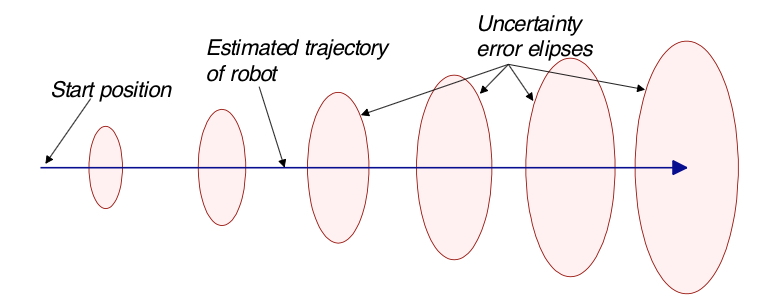
\includegraphics[width=.90\textwidth]{images/ellipses.jpeg}
\caption{Ellipses, depicting robot's position error, grow as odometry uncertainty increases}
\end{figure}

\subsection{Measuring Systematic errors}
Before describing Borenstein and Feng's method to estimate systematic errors, it is useful to analyse Borenstein and Koren's method (1987). \\
Let's suppose that robot starts its path from an initial position <$x_0, y_0, \theta_0$> and has to move on a 4x4 meter square path (Figure 2.2). The robot is programmed to return to its initial position at the end of the path, but because of systematic errors, this will not happen accurately and a series of errors will be accumulated (\emph{return position errors}):
\begin{equation}
	\begin{aligned}
		\epsilon_{x} &= x_{abs}-x_{calc} \\
		\epsilon_{y} &= y_{abs}-y_{calc} \\
		\epsilon_{\theta} &= \theta_{abs}-\theta_{calc}
	\end{aligned}
\end{equation}

We have denoted with the $abs$ subscript the absolute position and orientation of the robot and with $calc$ subscript the position and orientation of robot according to odometry.

This kind of experiment is not suitable for testing odometry for differential drive platforms. That is why Borenstein and Feng introduced their \emph{bidirectional square-path} experiment. This time, the robot is required to walk the path both in clockwise and counterclockwise direction. The errors $E_d$ and $E_b$ could compensate each other when robot travelled on one direction only; now, travelling on both direction, the two errors sum up.

If we let the robot travel on both directions $n$ times (usually, $n=5$), at the end of each run robot will accumulate a pose error as explained in (2.7). We can compute the center of gravity of these errors according to the following relations:
\begin{equation}
	\begin{aligned}
		x_{cg}^{cw} &= \frac{1}{n}\sum^n_{i=1}\epsilon_{x,i}^{cw} \\
		y_{cg}^{cw} &= \frac{1}{n}\sum^n_{i=1}\epsilon_{y,i}^{cw} \\
		x_{cg}^{ccw} &= \frac{1}{n}\sum^n_{i=1}\epsilon_{x,i}^{ccw} \\
		y_{cg}^{ccw} &= \frac{1}{n}\sum^n_{i=1}\epsilon_{y,i}^{ccw} 
	\end{aligned}
\end{equation}
The two absolute offsets of centers of gravity from origin are:
\begin{equation}
	\begin{aligned}
		r_{cg}^{cw} &= \sqrt{(x_{cg}^{cw})^2+(y_{cg}^{cw})^2} \\
		r_{cg}^{cw} &= \sqrt{(x_{cg}^{ccw})^2+(y_{cg}^{ccw})^2}
	\end{aligned}
\end{equation}
Finally, a measure of systematic odometric error can be obtained as
\begin{equation}
	E_{sys} = \max(r_{cg}^{cw},r_{cg}^{ccw}).
\end{equation}
The orientation error $\epsilon_\theta$ is not considered in $E_{sys}$, since each orientation error translates into a position error.
\begin{figure}[htbp]
\centering
\centering\setlength{\captionmargin}{0pt}%
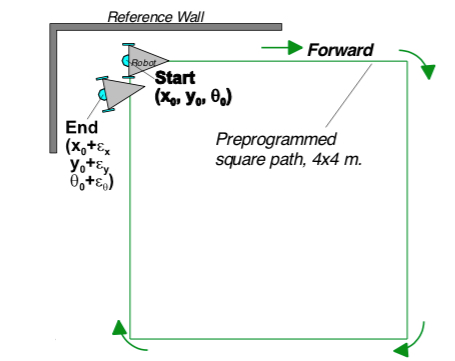
\includegraphics[width=.50\textwidth]{images/unidirectional_nominal_path.jpeg}
\caption{The 4x4 meter square path for Borenstein and Koren's method}
\end{figure}

\subsection{Measuring non-Systematic errors}
The square path test that was used to estimate systematic error, can be implemented again for non-systematic case, adding to the path some artificial bumps. Since return errors are sensible to the positions of bumps, this time error $\epsilon_\theta$ will be used. We can, then, compute an \emph{average absolute orientation error}:
\begin{equation}
	\epsilon_{\theta, avg}^{nonsys} = \frac{1}{n}\sum_{i=1}^{n}|\epsilon_{\theta,i, cw}^{nonsys}-\epsilon_{\theta,i, cw}^{sys}| + \frac{1}{n}\sum_{i=1}^{n}|\epsilon_{\theta,i, ccw}^{nonsys}-\epsilon_{\theta,i, ccw}^{sys}|
\end{equation}
The use of absolute values in previous equations is needed to avoid that two return orientation errors with opposite signs compensate each other. Thus, if after first run we have $\epsilon_\theta=1^\circ$ and after second one we have $\epsilon_\theta = -1^\circ$, we will not erroneously derive that $\epsilon_{avg}^{nonsys}=0^\circ$.

\section{Extracting features}
In many different fields (machine learning and pattern recognition, just to mention a pair) the amount of data to manage (for example, the measurements returned by robot sensor) is too huge to be used in toto, so it becomes of great importance to extract only the necessary information, removing, moreover, all the redundancies that could make computation unfeasible. Thus., it is convenient to design processes that are able to extract information that is representative of data and allows to overcome the problem of using data in its totality. Such processes perform what is called \emph{features extraction}, i.e. they retrieve (and sometimes compute) elements (\emph{features}) that are distinctive of data, with which it is easier to operate; features are required to be informative, discriminative and indipendent. For some uses, features are even required to mantain some properties across space and time. \\
Usually, features have a numerical nature, but sometimes they can present a different aspect (in some cases they can be strings of characters or histograms).

Before designing an extraction process, features' structure needs to be planned, in order to respect the goal of good representation of data and to obtain elements with which working will be easy and effective.
The choice about structure and computation of features depends on their final use and algorithms' purposes; here is a short list of common choices made in different fields:
\begin{itemize}
	\item{histograms of the distribution of black pixels in characters recognition}
	\item{phonemes in speech recognition}
	\item{repetitive words or text structures in spam detection, inside email inboxes}
	\item{edges and corners in computer vision}
\end{itemize}

As explained in previous section, data retrieved from odometry are often inaccurate and they can lead to errors in robot's position estimation; features, after their extraction from sensors' data, can add a precious information allowing to reduce the errors and gain a better estimate of robot position in time. Indeed, each feature carries information about its reciprocal position with respect to robot and it can be used to improve localization methods\\
It is necessary to underline that even a well designed process of extraction can return a number of features that is too huge to be handled; so, it becomes crucial, in such cases, to be aware about which features are really necessary and which can be ignored. This mainly depends on the context in which robot operates, the perception system and the way features are represented.

\subsection{Extracting lines as features}
On deciding which features need to be extracted, geometric primitives are always a good solution to the problem; in particular, lines are the simplest choice, since most environments can be described using line segments.
When receiving data from a ranger sensor (for instance, a laser range), one needs to operate with pairs $(\rho_i, \theta_i)$, which denote the position of i-th point in space, in polar coordinates, in robot's reference frame. Retrieving features from such information can be performed in two different ways:
\begin{itemize}
	\item{use a subset of points as features}
	\item{extract lines from the sequence of points, representing the part of environment seen by sensor during last scan}
\end{itemize}
For the purpose of this thesis, we will consider the second option.

Across the years, many algorithms have been developed for extracting lines, starting from a laser's sequence of points, each with its pros and cons. The choice of an algorithm instead of another one depends mainly on one's needs. Sometimes speed needs to be preferred, in some other cases it is preferrable to give importance to quality, since bad extraction of features may lead to system's divergence. Complexity, too, is a particular not to be forgotten. \\ 
Here, we will describe the so-called \emph{split and merge algorithm}, which operates using a \emph{divide et impera} logic, starting with an initial set of points, progressively divided into subsets (on the basis of a check condition), until satisfying the conditions for determining the existence of a line (the subset under inspection has not enough points to be divided into two subsets and/or no point satisfies check condition to proceed to another division).
The main steps of procedure are described by Algorithm 1. In particular:
\begin{itemize}
\item{\emph{isThereASetToSplit}($\mathcal{L})$ checks whether there is still a subset of points, among the ones in $\mathcal{L}$, that may be splitted into two subsets}
\item{\emph{takeASetToSplit($\mathcal{L}$)} extracts a set $s_i$ among the candidates to be splitted in $\mathcal{L}$}
\item{\emph{fitALine}($s_i$) returns a segment $l_i$ that best fits the points in $s_i$ (a simple choice may be computing the segment connecting the first and last point in $s_i$)}
\item{\emph{findFarthestPoint}($l_i$, $s_i$) returns the furthest point $P$ from $l_i$, among the ones in $s_i$}
\item{\emph{split}($s_i$, $P$) splits the set of points $s_i$ into two subsets: the first set contains the point preceeding $P$, the second one contains all remaining points}
\item{\emph{mergeCollinearLines}($\mathcal{L}$) merges segments that are collinear (i. e. segments that are very close to each other and lie on the same line)}
\end{itemize}
\begin{algorithm}
\caption{Split and merge algorithm}\label{euclid}
\begin{algorithmic}[1]
\item{\textbf{Input}: a set of all points $s_1$, an initially empty list $\mathcal{L}$ and a distance threshold $d_p$}
\item{\textbf{Output}: extracted segments (represented by their two extremes)}
\item{$\mathcal{L} \cup s_1$}
\item{\textbf{while}(\emph{isThereASetToSplit}($\mathcal{L})$)}
\item{\qquad $s_i$ = \emph{takeASetToSplit($\mathcal{L}$)}}
\item{\qquad $l_i$ = \emph{fitALine}($s_i$)}
\item{\qquad $P$ = \emph{findFarthestPoint}($l_i$, $s_i$)}
\item{\qquad \textbf{if}(\emph{distance(P, $l_i$)} > $d_p$)}
\item{\qquad \qquad ($s_j$, $s_k$) = \emph{split}($s_i$, $P$)}
\item{\qquad \qquad $\mathcal{L} \leftarrow \mathcal{L} - \{s_i\}$}
\item{\qquad \qquad $\mathcal{L} \cup \{s_k, s_j\}$}
\item{\emph{mergeCollinearLines}($\mathcal{L}$)}
\end{algorithmic}
\end{algorithm}

\section{Least squares estimation}
Let \textbf{x} be a vector variable indicating the state of the system and let's suppose to have a series of  functions 
\begin{equation}
	\{f_i(\textbf{x})\}_{i = 1:n} \notag
\end{equation}
which, given \textbf{x}, predict its measurement. \\Let's suppose, moreover, to have a series of real measurements ${\bf z_i}$. The goal is to extimate the state ${\bf x}$ that best fits the measurements ${\bf z_{i:n}}$.\\
We can, then, determine an error between each real measurement and the relative predicted one:
\begin{equation}
	\textbf{e}_i = \textbf{z}_i - f_i(\textbf{x})
\end{equation}
This error is assumed to be zero mean and normally distributed with information matrix \textbf{$\Omega_i$}. \\
If we compute the squared form of error, we notice that it is a scalar and depends only on the state of the system:
\begin{equation}
	e_i(\textbf{x}) = \textbf{e}_i(\textbf{x})^T\Omega_i\textbf{e}_i(\textbf{x})
\end{equation}
Then, the problem of finding the state that best fits the real measurements can be reduced to find the state ${\bf x^*}$ such that
\begin{align}
	\textbf{x*} &= \underset{\textbf{x}}{\mbox{argmin}} \enspace F(\textbf{x}) \\ \notag
	&= \underset{\textbf{x}}{\mbox{argmin}} \sum_i e_i(\textbf{x}) \\ 
	&= \underset{\textbf{x}}{\mbox{argmin}} \sum_i  \textbf{e}_i^T(\textbf{x})\Omega_i\textbf{e}_i(\textbf{x}) \notag
\end{align}
A general solution to the problem is to derive the global error function and find its nulls, but this would result in a complex solution which doesn't admit closed forms. So, proceeding with numerical approaches is a more practical path. 

If a good initial guess is at disposal and the measurement functions are smooth in the neighborhood of minima, we can solve problem using iterative (local) linearizations. The iterative process is composed of three steps:
\begin{itemize}
	\item{linearize the problem around current initial guess}
	\item{solve a linear system}
	\item{compute a set of increments to be applied to current estimate in order to get closer to minima}
\end{itemize}
The first step is linearizing the problem and this can be done using a Taylor expansion:
\begin{align}
	\textbf{e}_i(\textbf{x} + \Delta\textbf{x}) &\simeq \textbf{e}_i(\textbf{x}) + \frac{\partial \textbf{e}_i}{\partial \textbf{x}}\Delta\textbf{x}\\
	&= \textbf{e}_i + \textbf{J}_i\Delta\textbf{x} \notag
\end{align}
We can now place the Taylor expansion in the squared error:
\begin{align}
	&e_i(\textbf{x} + \Delta\textbf{x}) \simeq \notag \\
	&\textbf{e}_i^T\Omega_i\textbf{e}_i + \textbf{e}_i^T\Omega_i\textbf{J}_i\Delta\textbf{x} + \Delta\textbf{x}^T\textbf{J}_i^T\Omega_i\textbf{e}_i + \Delta\textbf{x}^T\textbf{J}^T_i\Omega_i\textbf{J}_i\Delta\textbf{x} \notag \\
	&= \underbrace{\textbf{e}_i\Omega_i\textbf{e}_i}_\text{$c_i$} + 2\underbrace{\textbf{e}_i^T\Omega_i\textbf{J}_i}_\text{$b_i^T$}\Delta\textbf{x} + \Delta\textbf{x}^T\underbrace{\textbf{J}_i^T\Omega_i\textbf{J}_i}_\text{$\textbf{H}_i$}\Delta\textbf{x} \notag \\
	&= c_i + 2\textbf{b}_i^T\Delta\textbf{x} + \Delta\textbf{x}^T\textbf{H}_i\Delta\textbf{x}
\end{align}
The global error is the sum of the squared errors, so, from (3) and (5), we have:
\begin{align}
	F(\textbf{x} + \Delta\textbf{x}) &\simeq \sum_i(c_i + 2\textbf{b}_i^T\Delta\textbf{x} + \Delta\textbf{x}^T\textbf{H}_i\Delta\textbf{x}) \notag \\
	&= \sum_i c_i + 2(\sum_i\textbf{b}_i^T)\Delta\textbf{x} + \Delta\textbf{x}^T(\sum_i\textbf{H}_i)\Delta\textbf{x}
\end{align}
where
\begin{align}
	\textbf{b}^T &= \sum_i\textbf{e}_i^T\Omega_i\textbf{J}_i  \\
	\textbf{H} &= \sum_i\textbf{J}_i^T\Omega_i\textbf{J}_i 
\end{align}
The expression of global error we have just obtained is quadratic in $\Delta\textbf{x}$ and can be minimised; for this purpose, we can compute its derivative with respect to $\Delta\textbf{x}$ in the neighbourhood of current solution $\textbf{x}$:
\begin{equation}
\frac{\partial F(\textbf{x}+\Delta\textbf{x})}{\partial\Delta\textbf{x}} \simeq 2\textbf{b} + 2\textbf{H}\Delta\textbf{x}
\end{equation}
with the optimal solution reached for 
\begin{equation}
\Delta\textbf{x*} = -\textbf{H}^{-1}\textbf{b}
\end{equation}
Thus, an iterative algorithm can be designed; it will execute the following steps:
\begin{itemize}
	\item{linearize the system around current guess $\textbf{x}$ and compute $\textbf{e}_i(\textbf{x} + \Delta\textbf{x})$ as described in () and ()}
	\item{compute $\textbf{b}^T$ and $\textbf{H}$ as described in () and ()}
	\item{solve the system to get a new optimal increment $\Delta\textbf{x*}$, as indicated in ()}
	\item{update the previous estimate: $\textbf{x} \leftarrow \textbf{x} + \Delta\textbf{x*}$}
\end{itemize}

% -------------------------------------------------------------------------------

\chapter{Fast Position Tracking: overall approach}

\section{Introduction}
As stated in previous sections, the amount of information returned by sensors is often too huge to be handled; thus, it is opportune to extract only relevant part that, in the case of laser scans, is in the form of lines, expressed in their polar representation. The set of lines furnishes a glimpse of environment's aspect, through the use of a \emph{polyline structure}, which reflects how ambient has been seen by robot.

Given the lines obtained from each scan, it becomes interesting to track how the same line moves across scans and to recognise the same line in two (or more) different robot's perceptions: such problem, can be afforded using a new representation for lines, based on their normals and midpoints; this new representation, coupled with a least square minimisation approach, allows to design an iterative process that corrects, progressively, the estimate of a transformation matrix between two scans. When the final transformation $T$ has been returned, it can be used to map the lines of a scan into another and determine associations between the lines revealed as the same across the two perceptions.



\section{Landmarks and features}
As discussed in last chapters, once a robot has acquired information from a sensor (a laser scan, for instance), it is necessary to extract only the relevant part of data, in order to reduce complexity without affecting performances. Such relevant part is formed by \emph{features}, elements that describe reliably the part of environment perceived by a sensor's acquirement. They may represent physical objects and in robotics are often called \emph{landmarks}, to underline the fact that they are exploited by robot during navigation. Without losing generality, we can assume that robot is always able to measure the bearing and range of landmarks in its own reference frame (Figure 3.1). Sometimes, an extractor adds a \emph{signature} to measurements, in terms of a numerical value that can represent, for instance, an average color. The presence of signature is not strictly required and all what will be exposed in the following can be reduced to the case in which no signature has been introduced.

If we denote with $f$ an extractor function, the extracted features can be represented as $f(z_t)$; let's indicate with $r$, $\phi$ and $s$ the range, the bearing and the signature. We can obtain, then, a feature vector as a collection of triplets:
\begin{equation}
	f(z_t) = \{f_t^1, f_t^2, \dots \} =\left \{ \left( \begin{matrix} r_t^1 \\ \phi_1^t \\ s_t^1 \end{matrix} \right),  \left(\begin{matrix} r_t^2 \\ \phi_2^t \\ s_t^2 \end{matrix} \right), \dots \right\}
\end{equation}
It is commonly accepted that features are independent from each other; such independence can be formalised as
\begin{equation}
	p(f(z_t) \: | \: x_t, m) = \prod_i p(r_t^i, \phi_t^i, s_t^i \: | \: x_t, m)
\end{equation}
where $m$ is the map computed up to time instant $t$ and $x_t$ is current robot's state. \\
Actually, independence between features can be guaranteed only if the noise on a measurement $(r_t^i, \phi_t^i, s_t^i)$ is independent from the noise on another measurement $(r_t^j, \phi_t^j, s_t^j)$; when independence can be assumed, each feature can be processed separately and it is possible to design more efficient algorithms to implement probabilistic measurement models. 

For feature-based algorithms, the map $m$ is composed by a collection of features $m = \{m_1, m_2, \dots \}$. To each feature on the map corresponds a \emph{location coordinate}, whose components can be denoted by $(m_{i,x} \quad m_{i,y})$. Assuming that, at time $t$, the $i$-th feature corresponds the $j$-th landmark and that robot's state, at the same instant, is described by $x_t = (x \quad y \quad \theta)$, we can model noise on measurement:
\begin{equation}
	\left(\begin{matrix} r_t^i \\ \phi_t^i \\ s_t^i	\end{matrix} \right) = \left( \begin{matrix} \sqrt{(m_{j,x} - x)^2 + (m_{j,y} - y)^2} \\ \mbox{atan2}(m_{j,y} - y, m_{j,x}-x) - \theta \\ s_j\end{matrix}\right) + \left( \begin{matrix}\epsilon_{\sigma_r^2} \\ \epsilon_{\sigma_{\phi}^2} \\ \epsilon_{\sigma_s^2}\end{matrix}\right)
\end{equation}
where $\epsilon_{\sigma_r^2}$, $\epsilon_{\sigma_\phi^2}$ and $\epsilon_{\sigma_s^2}$ are zero-mean Gaussian error variables with variances $\sigma_r^2$, $\sigma_\phi^2$ and $\sigma_s^2$, respectively.

\begin{figure}[htbp]
\centering
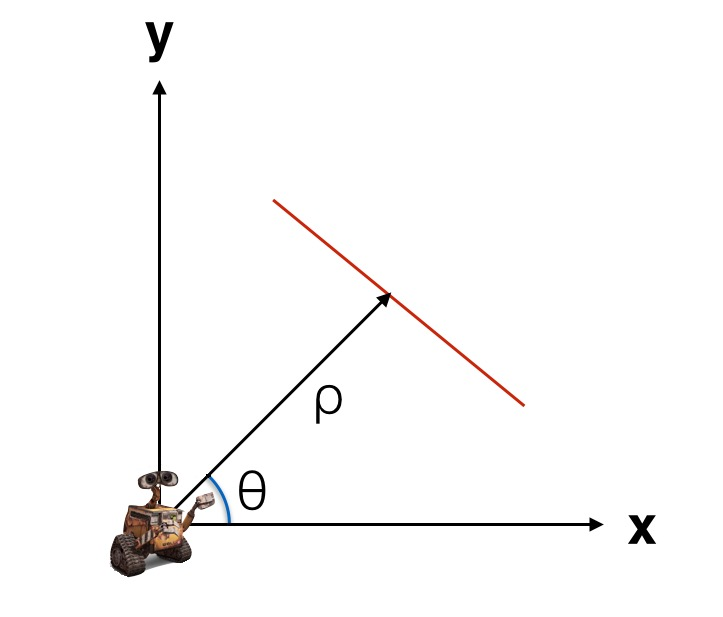
\includegraphics[width=.50\textwidth]{images/rho_theta.jpeg}
\caption{The range $\rho$ and the bearing $\theta$, relative to a landmark (line), expressed in robot's reference frame}
\end{figure}

\subsection{Extraction and model of features}
When working with 2D landmarks, line segments represent a good choice for determining a reliable set of features, since they are simple geometric primitives but, at the same time, furnish a good amount of information to be used during localisation phases. The easiest way to represent a segment is by its endpoints; in some circumstances (for instance, the cases in which a robot scans an environment in which different corridors share a wall), the endpoints' information may be misleading, but the distance that can be measured between them is, at the least, a lower bound on the actual length of the segment they delimit.

Given a scan from laser, the \emph{Split and merge} algorithm described in Section 2.4.1 can be used to extract segments, which can be characterised by their endpoints. When segments appear to be collinear and their extremes are close enough, they can be melted or joined, obtaining what is known as a \emph{polyline structure}. Segments that could not be joined and whose length falls below a determined threshold, can be deleted, since they represent a useless source of noise. It is, moreover, possible to gain a polar representation of segments, using the aforementioned equation 
\begin{equation}
	x\cos \theta + y\sin\theta = \rho, \notag 
\end{equation}
where $\rho$ is the distance of line from the origin and $\theta$ is its orientation, in terms of its slope with respect to $x$ axis. Both quantities are expressed in robot's reference frame.

\section{Matching features}
If we consider two scans $i$ and $j$ returned by robot's laser, according to previous section, we are able to extract lines from each of them, elaborate them and obtain a polyline structure formed by extracted segments. \\
What becomes of great interest at this moment is discovering whether one or more lines in scan $i$ correspond to lines extracted from scan $j$. This is what is known as the \emph{matching problem}. \\
Finding out the associations between lines belonging to different scans allows to compute a rigid transformation $T$ from scan $j$ to scan $i$; such transformation, is actually able to translate the reference frame of robot in which $j$ was acquired onto reference frame in which $i$ was expressed. The sought transformation should be able to maximize the overlapping between the two reference frames, minimising, at the same time, the value of an opportune error function.

\subsection{Solving matching problem using least squares estimation}
The problem of determining $T$ can be formulated in terms of a least square estimation, by exploiting the concepts in Section 2.5. Let's suppose that a generic segment $l_i$ in scan $i$ can be expressed as 
\begin{equation}
	l_i = \left(\begin{matrix} p_i \\ n_i \end{matrix} \right)
\end{equation}
where $p_i$ is a point on segment (middlepoint is the most convenient choice) and $n_i$ is segment's normal, in its classical expression
\begin{equation}
	n_i = (\cos\theta_i \quad \sin\theta_i)^T.
\end{equation}
The needed transformation T will always have the form
\begin{equation}
	T = \left(\begin{matrix} R && \bf{t} \\ \bf{0} && 1 \end{matrix}\right)
\end{equation}
where $R$ is a $2\times2$ rotation matrix, \textbf{t} is traslation vector and \textbf{0} is a $1\times2$ zero vector. We can assume an initial value for $T$: in particular, $T$ can assume the value of an initial guess or can be simply set to a $3\times3$ identity matrix. The transformation embodied by initial $T$ can be applied to $l_i$, obtaining a new line $l'$:
\begin{equation}
	l' = Tl_i = \left(\begin{matrix}Rp_i+t \\ Rn_i\end{matrix}\right)
\end{equation}
As it is evident from previous expression, to the generic point on segment a roto-traslation is applied, while only a rotation is applied to segment's normal. Supposing that new segment $l'$ should be matched, after applying transformation, with a line $l_j = (p_j \quad n_j)^T$ in scan $j$, we can define an error function
\begin{equation}
	e_{ij}(T) = \left(\begin{matrix}Rp_i + \textbf{t} - p_j \\ Rn_i - n_j \end{matrix}\right)
\end{equation}
A perturbation $\Delta T$ can be introduced to the error function, determining a new function
\begin{equation}
	e_{ij}(T \oplus \Delta T) = \left(\begin{matrix} \Delta R(Rp_i + \textbf{t}) + \Delta T - p_j \\ \Delta R \cdot Rn_i - n_j \end{matrix}\right)
\end{equation}
Deriving previous expression, we get:
\begin{equation}
	\frac{\partial e_{ij}(T \oplus \Delta T)}{\partial \Delta T} = \left(\begin{matrix} \textbf{I}_{2 \times 2} \\ \\ \textbf{0}_{2 \times 2} \end{matrix} \quad \begin{matrix} -p_{iy} \\ p_{ix} \\ -n_{iy} \\ n_{ix}\end{matrix}\right) = J_{ij},
\end{equation}
where subscripts $ix$ and $iy$ indicate the components $x$ and $y$ in $p_i$ and $n_i$.

If we were able to rotate a single segment, in such a way its normal is parallel to $x$ axis, we could obtain the useful result of having the segment's variance only moving along $x$. This result can be achieved by defining a covariance matrix as
\begin{equation}
	\Omega_{ij} = \left(\begin{matrix} \Omega_{p_i} && \textbf{0}_{2\times2} \\ \textbf{0}_{2\times2} && \alpha \textbf{I}_{2\times2} \end{matrix}\right)
\end{equation}
with
\begin{equation} \Omega_{p_i} = R_i\left(\begin{matrix} 1 && 0 \\ 0 && \epsilon \end{matrix}\right)R_i\end{equation}
and
\begin{equation}
	R_i = \left(\begin{matrix} n_{ix} && -n_{iy} \\ n_{iy} && n_{ix} \end{matrix} \right).
\end{equation}
The constants $\alpha$ and $\epsilon$ are chosen in such a way they have small values.

Once covariance matrix $\Omega_{ij}$ has been computed, we can proceed to define an iterative process that permits to update the current value of transformation $T$. We first operate locally, according to equations
\begin{equation}
	\begin{aligned}
		H_{ij} &= J_{ij}^T\Omega_{ij}J_{ij} \\
		b_{ij} &= J_{ij}^T\Omega_{ij}e_{ij}.
	\end{aligned}
\end{equation}
Then, we operate globally:
\begin{equation}
	\begin{aligned}
		H &= \sum_{ij} H_{ij} \\
		b &= \sum_{ij} b_{ij}
	\end{aligned}
\end{equation}
Using global matrices, we can solve system 
\begin{equation}
	H\Delta T^\star = b
\end{equation}
and obtain a new value $T_{\mbox{new}}$ for the current estimate of transformation, according to
\begin{equation}
	\begin{aligned}
		T_{\mbox{new}} &= \mbox{toMatrix}(\Delta T)^\star \cdot T \\
		T  &\leftarrow  T_{\mbox{new}} 
	\end{aligned}
\end{equation}
where \emph{toMatrix} is a function that builds a transformation matrix, starting from vector $\Delta T$, containing displacements along axes and rotation value.

\subsection{Determining associations between features}
All what has been explained in previous section, can be inserted in an iteration process that tends to reduce progressively the error in alignment between two frames, while trying to find the transformation $T$ to map one into the other. \\
Let's suppose to have two scans $i$ and $j$ and that we need to find the transformation $T$ from $j$ to $i$; let's suppose, moreover, to have chosen an initial value for $T$ and a maximum number of iterations $N$. The steps of iteration process are summarised in the following.

\textbf{Applying current transformation $T$}. The first action is applying $T$ to all the lines in $j$, in order to map them into reference frame $i$. As underlined previously, we can have an initial guess or an identity matrix as transformation, at first iteration of the process. Subsequently, we will apply, at iteration $k$, the transformation we obtained at $k-1$.

\textbf{Data association}. The lines that have just been transformed need to be associated to lines in $i$. First, we try to form associated couples by comparing each transformed lined with the ones in $i$ and finding the closest one comparing the normals. In particular, given the normals $n_i$ and $n_j$ of line $l_i$ and transformed line $l_j$, respectively, we compute the dot product
\begin{equation}
	p_{ij} = n_i^Tn_j
\end{equation}
Then, we add to a set the couple of associated indexes $(i, j)$ if $p_{ij}$ is greater than a properly chosen threshold. This gives us a set of putative associations that needs to be pruned. \\
Lately, for each couple of indexes, we evaluate the difference between the values of $\theta_i$ and $\theta_j$ of associated lines, along with the Euclidean distance between their midpoints. Both are requested two stay below two specific thresholds. All the couples of indexes, whose associated lines don't satisfy these last two conditions, are deleted from putative set. 

\textbf{Computing local and global matrices}. Once we have a set of reliable couples of indexes (lines), for each couple we can compute the error $e_{ij}$ as expressed in Equation (3.9); this allows us to determine the local matrices $H_{ij}$ e $b_{ij}$ (Equations from 3.9 to 3.14), for each couple of associated lines. Once all local matrices have been computed, we can derive global matrices $H$ and $b$ (Equations 3.15).

\textbf{Solving linear system and updating current estimate of $T$}. Once the global matrices have been computed, it is possible to prepare linear system in (3.16). Its resolution gives us the new estimate $\Delta T$ of transformation matrix between scans $i$ and $j$.  By applying new estimate to old one, we get a new transformation matrix that can be used for a new iteration of algorithm or can be directly returned if the maximum number of iterations has been reached. A block representation of a single iteration can be found in Figure 3.2.

\begin{figure}[htbp]
\centering
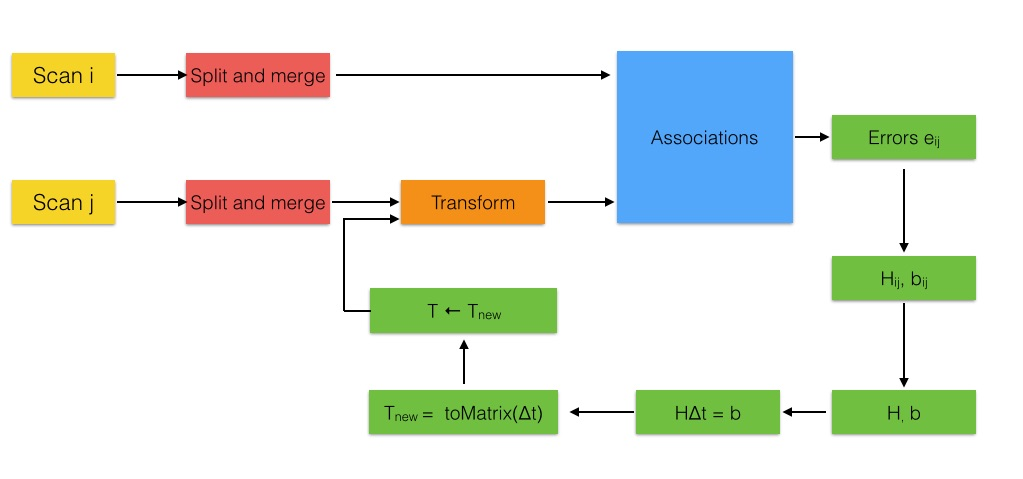
\includegraphics[width=1\textwidth]{images/iterative_process.jpg}
\caption{Block representation of a single iteration in $T$ estimation}
\end{figure}

\chapter{Experiments}
\section{Introduction}
This chapter deals with some tests designed to evaluate two of the parts composing thesis: the least square estimation (LSE) module and the one performing data association. Before going into deep of tests, the reader will be introduced to the main means used for evaluation: the Robot Operating System and its embedded module \emph{Stage}, used to generate data and simulations.

\section{Robot Operating System}
According to Willow Garage, the research laboratory that developed it in 2007, the \textbf{Robot Operating System} (\textbf{ROS}) can be defined as a \emph{flexible framework for writing robot software}. Actually, ROS can be thought of as a collection of frameworks that can be exploited for the development of robot's software; such collection, furnishes all the typical functionalities of an operating system,  along with robot-oriented capabilities. Here is a short list:
\begin{itemize}
	\item{hardware abstraction}
	\item{low-lovel device control}
	\item{exchange and recording (in \emph{bag files}) of messages between processes}
	\item{robot-specific features: pose estimation, localisation, mapping, navigation (Figure 4.1)}
	\item{diagnostics, to produce, collect and aggregate data about robot, to control its state and produce an effective strategy to resolve incoming issues}
	\item{tools for debugging, plotting, and visualizing the state of the system under development (Figure 4.2)}
	\item{package management}
\end{itemize}

\begin{figure}[htbp]
\centering
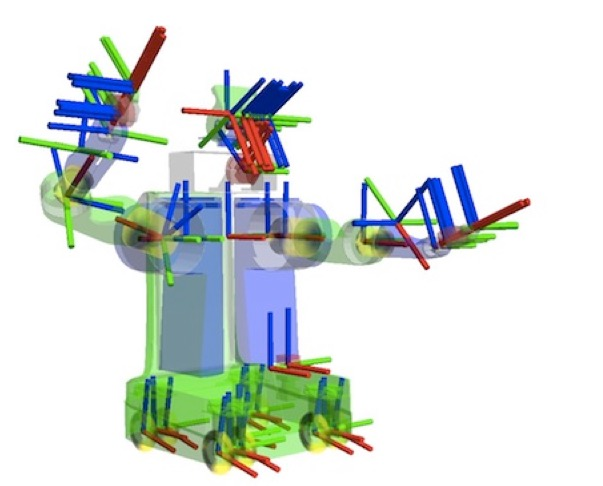
\includegraphics[width=.90\textwidth]{images/tf.jpeg}
\caption{An example of robot-specific features: the \emph{tf} library, which tracks the position of different elements of robot (sensors, links) in the robot's reference frame}
\end{figure}

Mainly, ROS' aim is simplifying the task of designing robot's behaviour across different platforms. It has been built in a collaborative mood, since it is open source and counts on the work of different developers and institutions to enrich the basic functionalities.\\
ROS-based applications are organised in a graph structure composed of \emph{nodes}, in which processes are executed and can receive or post messages regarding sensors, control, state, planning, actuators and so on. Even if a certain low latency is required in prevailing robotics, ROS is not a real time operating system, but it can be integrated with realtime code. 
\begin{figure}[htb]
\centering
\begin{minipage}[c]{0.6\textwidth}
\centering\setlength{\captionmargin}{0pt}%
\centerline{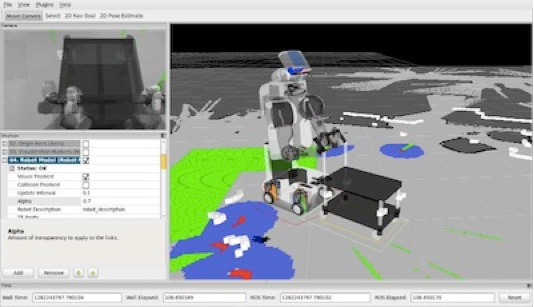
\includegraphics[width=1.5\textwidth]{images/rviz.jpeg}}
(a)
\end{minipage} \\
\vspace{10mm}%
\begin{minipage}[c]{0.6\textwidth}
\centering\setlength{\captionmargin}{0pt}%
\centerline{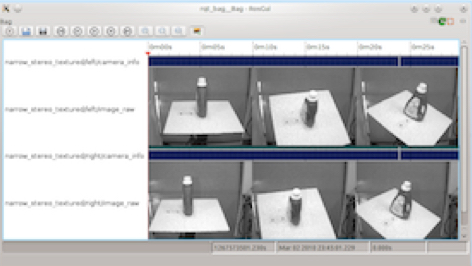
\includegraphics[width=1.5\textwidth]{images/rqt_bag.jpeg}}
(b)
\end{minipage}
\caption{Two examples of ROS tools. The \emph{rviz} tool (a) visualizes many common messages provided in ROS, such as laser scans, three-dimensional point clouds and camera images. It also uses information from the \emph{tf} library to show sensor data in a chosen coordinate frame, along with a three-dimensional rendering of robot. The \emph{ rqt\_bag} tool (b) records data to bags and can display their content.}
\end{figure}
There are, essentially, three kinds of softwares inside ROS:
\begin{itemize}
	\item{language and platform independent tools for ROS distribution and building, under BSD licence\footnote{The Berkeley Software Distribution (BSD) licence was originally created in 1990 to define the rules by which open source code can be used and distributed. The BSD licence requires the name of the code's developer to be always reported, even in documentation, along with a disclaimer specifying that code is released "as it is", without any garantee about its performance. The identities of contributors can't be used to endorse derived software, particularly for commercial purposes.}}
	\item{client library implementations (\emph{roscpp, rospy, roslisp}), under BSD licence}
	\item{custom code using client libraries, which is sometimes commercial and is released under various open source licenses}
\end{itemize}
The last category in previous list contains packages usually implemented for hardware drivers, robot models, perception, simultaneous localisation and mapping (SLAM).

\section{The ROS Stage Simulator}
In order to test the line extraction, the least square estimation and the data association between lines in different scans, it is necessary to generate real data by simulating the robot behaviour (scanning comprised) in a realistic environment. \\
When a real robot is not at the disposal, it is possible to simulate and make it move through the use of \emph{Stage} simulator, which provides a virtual world populated with other mobile robots, sensors and objects that robot can sense and manipulate. \emph{Stage} can be used as a stand-alone program or can be embedded inside a larger library or framework (we will use its embedded version inside a ROS node).\\
\emph{Stage} itself provides the models of a series of actuators and sensors (sonar, infrared rangers, scanning laser rangefinder, bumpers, grippers); it provides even the model of a variety of mobile robot bases with odometric or global localisation. 

To generate an accurate simulation in \emph{Stage}, two elements are strictly necessary:
\begin{itemize}
	\item{a map (\emph{world}) in which robot needs to move}
	\item{a player making robot move in simulated environment}
\end{itemize}

With regards to maps, \emph{Stage} furnishes a certain number of them that can be used to start learning how a simulation in its environment works. Anyway, for more specific uses it could be required to create the map of a specific ambient in which robot has to move and sense. The definition of a map requires the creation of three objects:
\begin{itemize}
	\item{a \emph{.png} file representing the shape of environment, created with the use of a laser rangefinder or by graphics editors (Figure 4.3)}
	\item{a \emph{.world} file, containing the description of ambient (dimension of map, robots' initial positions and colors). An example relative to Figure 4.3 is showm in Figure 4.4}
	\item{a \emph{.yaml} file, containing information, for instance, regarding the position of origin of axes on \emph{.png} file, that will be used as a reference to track robot's position along its trajectory (Figure 4.5)}
\end{itemize}
\begin{figure}[htbp]
\centering
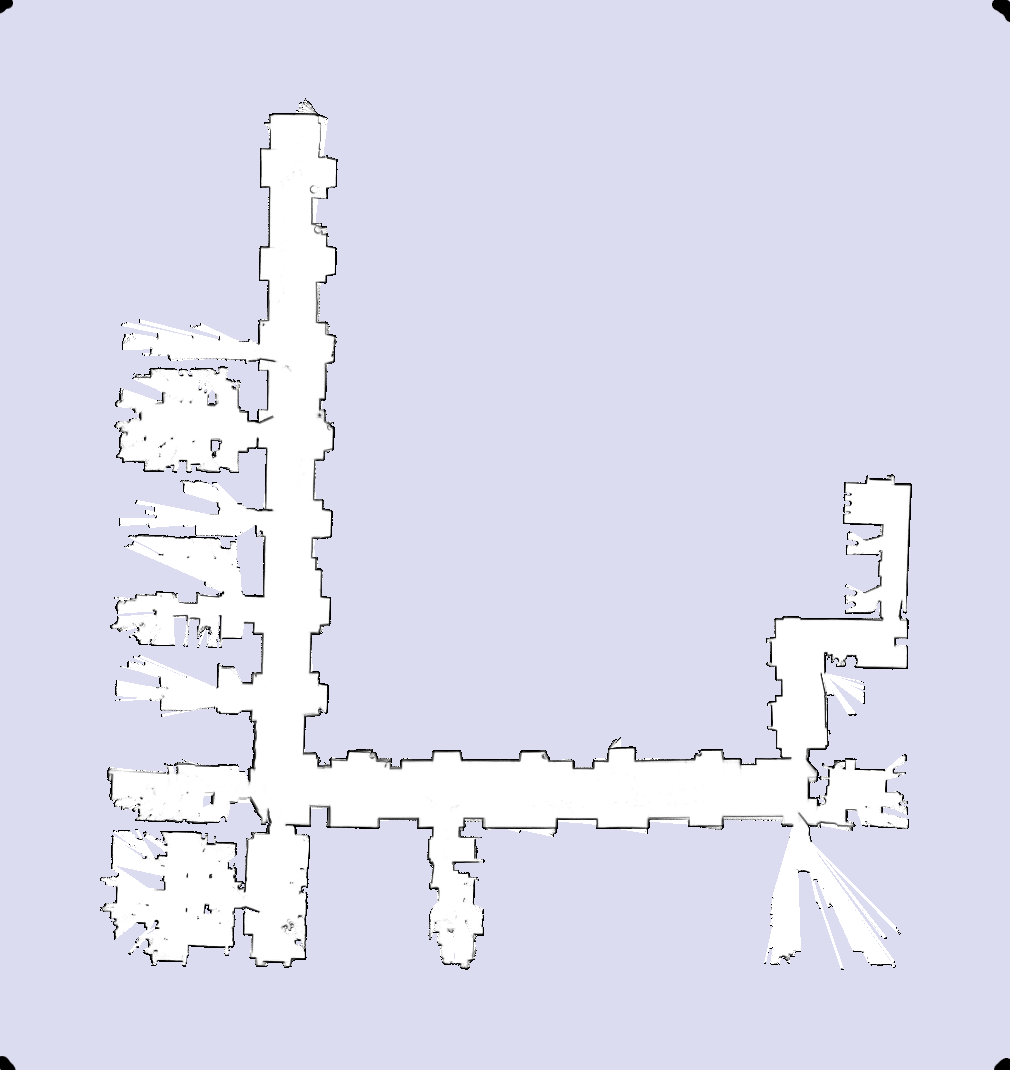
\includegraphics[width=1\textwidth]{images/mappa_dis/dis-B1-2011-09-27.png}
\caption{A \emph{.png} file created for the definition of a map in \emph{Stage}, depicting the first floor of DIAG department}
\end{figure}

\begin{figure}[htbp]
\centering
\fbox{
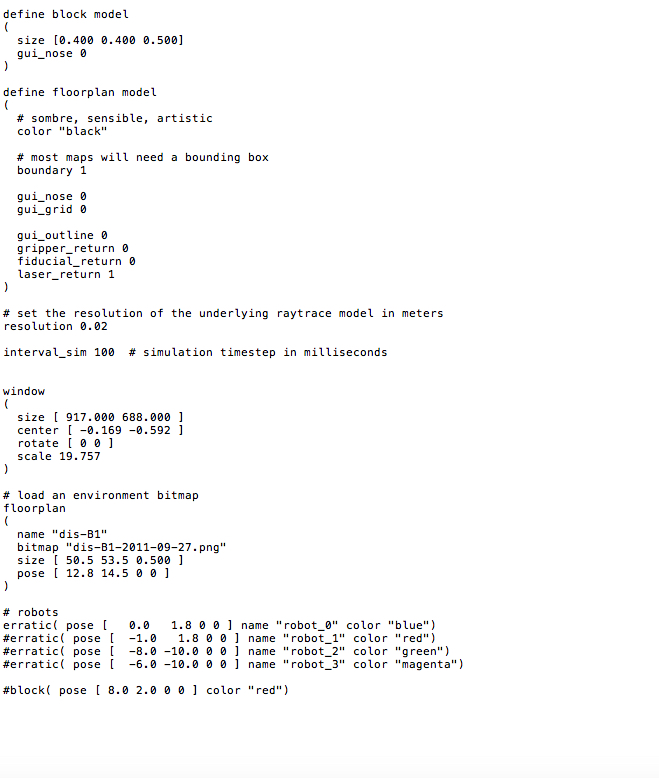
\includegraphics[width=1\textwidth]{images/mappa_dis/world_file.jpg}}
\caption{A \emph{.world} file relative to Figure 4.3}
\end{figure}

\begin{figure}[htbp]
\centering
\fbox{
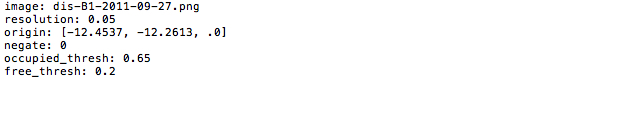
\includegraphics[width=1\textwidth]{images/mappa_dis/yaml_file.jpg}}
\caption{A \emph{.yaml} file relative to Figure 4.3}
\end{figure}

Each robot on the map is usually represented as a small square with a different color; to make it move forward (along X or Y axes) or rotate, it is necessary to use another external library contained in another ROS node. \\
There is not a unique option, but a good choice is \emph{teleop\_base}; such node exploits the system for messages exchange described in previous section. \emph{Teleop\_base} receives commands from keyboard (Figure 4.6) and generates a message about which movement robot on map has to perform (either a straight progression or a rotation) and sends it to \emph{Stage} simulator, which moves square associated to robot accordingly on the map.
\begin{figure}[htbp]
\centering
\fbox{
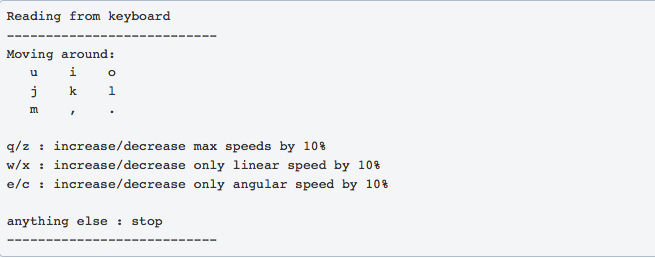
\includegraphics[width=1\textwidth]{images/mappa_dis/teleop_base.jpg}}
\caption{Keyboard commands used by \emph{teleop\_base} controller}
\end{figure}\\
\emph{Stage} itself is able to generate two kinds of messages:
\begin{itemize}
	\item{\emph{geometry\_msgs} which contain information about robot's position}
	\item{\emph{nav\_msgs} which contain information about data acquired by robot during its trajectory (usually in the form of couples $(\rho, \theta)$, describing the polar coordinates of points returned by range finder)}  
\end{itemize}
Such messages can be recorded in a \emph{bag file}, a kind of container that intercepts and stores messages of specified types; recorded messages can be played back and received by new addresses. The message system requires a sort of DNS server that knows sender and receiver of each message; \emph{roscore}, which can be executed from another ROS node, is the most natural choice for this purpose.

\section{Results}
In the following, it will be explained how some tests have been performed to evaluate the single parts forming the matter of this thesis; in particular, tests have been designed for the least squares and data association parts.
\subsection{Preliminaries}
All the testing activities that will follow, can be essentially divided into two parts:
\begin{itemize}
	\item{generation of testing data}
	\item{testing of overall approach}
\end{itemize}
For the generation of data, we used the \emph{Stage} simulator and the map of first floor of DIAG department, depicted in Figure 4.3. The robot, represented, as usually, as a small square, was made move for a short journey along one of the corridors, using \emph{teleop\_base} and keyboard commands. While robot was moving, \emph{Stage} generated \emph{geometry\_msgs} and \emph{nav\_msgs} messages, that were recorded in a bag file. \\
Subsequently, it was necessary to translate data in bag file into something more readable and useful for later uses; for such goal, an ad hoc ROS node was designed. Its task was listening to messages coming from the playback of bag file and record fundamental information on text files. In particular, the node extracted, from messages, information about odometric data and polar coordinates of scanned points, for each robot pose. The polar coordinates were converted in Cartesian coordinates (in robot's reference frame) before being saved on a text file.

The testing part was inserted in a separate ROS node; the node first loaded all the information previously recorded of text files, paying attention not to consider more than once the same pose and its associated data. From the points returned at each scan, lines were extracted using the \emph{split and merge} algorithm described in Chapter 1.

\subsection{Testing least squares estimation (LSE)}
The first and easiest test that can be performed on LSE module requires to take the lines extracted from a scan of robot (at a given pose), to apply them a chosen transformation and to verify whether the LSE can reconstruct the applied transformation, without knowing it a priori.
Let's suppose to have three small vectors, each one containing a series of movements along axes or rotations:
\begin{equation}
	\begin{aligned}
		S_x &= \{x_1 \quad x_2\} = \{ -5 \quad 0.5\} \\ \notag
		S_y &= \{y_1 \quad y_2\} = \{-0.3 \quad 7\} \\ \notag
		S_\theta &= \{\theta_1 \quad \theta_2\} = \left\{-\frac{3}{2}\pi \quad \frac{\pi}{6}\right\} \notag
	\end{aligned}
\end{equation}.

Using elements in these sets it is possible to determine a series of roto-translations 
\begin{equation}
	(x_i \quad y_j \quad \theta_k) \quad x,j,k \in [1,2] 
\end{equation}
given by all the possible combinations of three elements that can be obtained by picking an item in each set. Taking into account the generic roto-translation given by (5.1), we can construct a transformation matrix
\begin{equation}
	T = \left(\begin{matrix}\cos\theta_k && \sin\theta_k && x_i \\ -\sin\theta_k && \cos\theta_k && y_j \\ 0 && 0 && 1\end{matrix}\right)
\end{equation}
Our test of LSE module consists in taking a single scan, apply to all its lines the transformation $T^{-1}$ and verify whether LSE is able to return matrix $T$ as the one to bring converted lines to their original form. For each possible roto-translation, we showed lines before applying $T^{-1}$ (bold red), after its application (bold black) and after applying the resulting transformation matrix returned by LSE (yellow). We generated eight figures; Table 1 shows, for each figure, which combination, among the ones generically described in (5.1), was used for testing and produce plot. \\
What is evident is that LSE is always able to return a result very close to $T$; so, when LSE's returned matrix is applied to lines transformed with $T^{-1}$, we obtain, in practice, original scan's lines. This means that LSE algorithm always converges to a correct solution and it is always possible to retrieve the correct transformation to map lines from one transformed scan to original one.

A measure of how fine are LSE's performances, can be retrieved by remembering that LSE works with an initial set of lines couples; for each of them, it is possible to calculate the error $e_{ij}$ and covariance matrix $\Omega_{ij}$, according to equations 4.8 and 4.11. So, for each couple, an error measure is given by 
\begin{equation}
	e_{ij}\Omega_{ij}e_{ij}^T
\end{equation}
The quantities in (5.3) computed at $i$-th iteration of LSE can be summed, an error measurement $\chi_i$. Thus, after $N$ iterations, LSE returns a total local error
\begin{equation}
	\chi = \sum_i^N \chi_i
\end{equation}
For each figure listed in Table 5.1, we have shown how $\chi$ varies at each iteration of LSE (all the times, we executed LSE one hundred times). It is clear that $\chi$, although starting from high values, falls quickly to zero after a few iterations and maintains such value up to the end of LSE's execution, demonstrating its good performances. 


\begin{center}
\begin{table}
    \begin{tabularx}{\textwidth}{@{}lYYYYY@{}}
  \hline
\textbf{\#Figure} & \textbf{$x_i$} & \textbf{$y_j$} & \textbf{$\theta_k$}\\ \hline
\textbf{5.7} & -5 & -0.3 & $-3\pi/2$ \\ \hline
\textbf{5.8} & -5 & -0.3 & $\pi/6$ \\ \hline
\textbf{5.9} & -5 & 7 & $-3\pi/2$ \\ \hline
\textbf{5.10} & -5 & 7 & $\pi/6$ \\ \hline
\textbf{5.11} & 0.5 & -0.3 & $-3\pi/2$ \\ \hline
\textbf{5.12} & 0.5 & -0.3 & $\pi/6$ \\ \hline
\textbf{5.13} & 0.5 & 7 & $-3\pi/2$ \\ \hline
\textbf{5.14} & 0.5 & 7 & $\pi/6$ \\ \hline
   \hline
    \end{tabularx}
\caption{Roto-translation used for testing LSE and relative number of Figure}
\end{table}
\end{center}

\begin{figure}[htbp]
\centering
%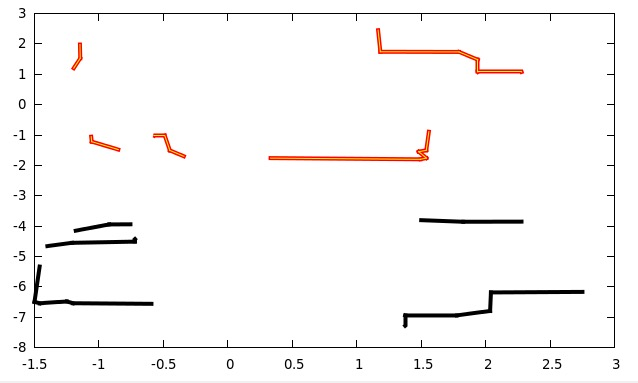
\includegraphics[width=1.0\textwidth]{images/foto_test/-5_-0.3_-4.7124/plot.jpeg}
%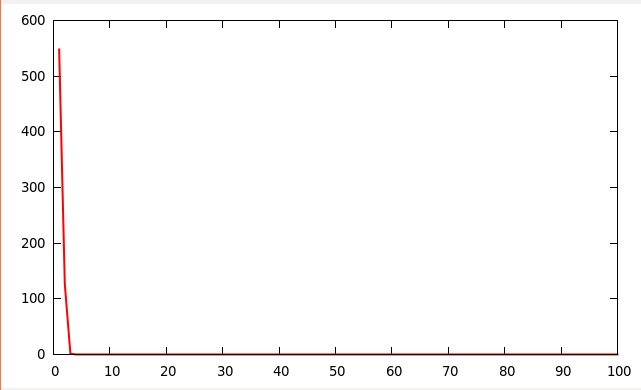
\includegraphics[width=1.0\textwidth]{images/foto_test/-5_-0.3_-4.7124/chi.jpeg}
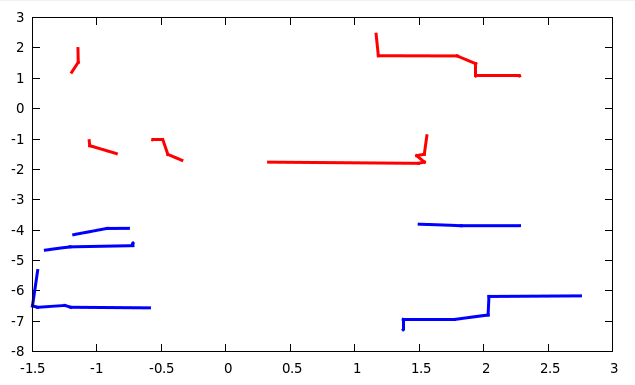
\includegraphics[width=0.9\textwidth]{images/foto_test/-5_-0.3_-4.7124/before_after.png}
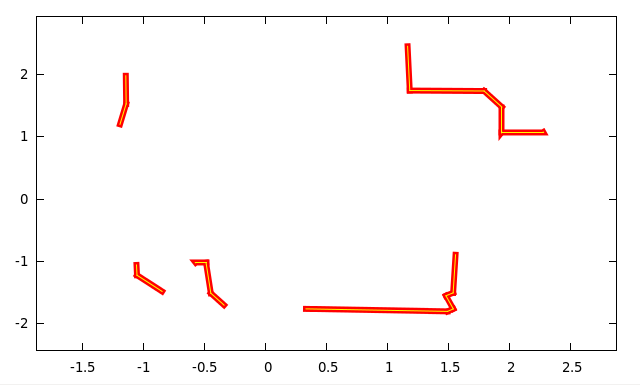
\includegraphics[width=0.9\textwidth]{images/foto_test/-5_-0.3_-4.7124/result.png}
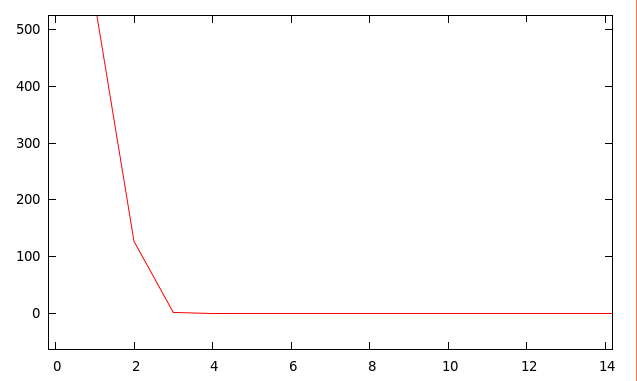
\includegraphics[width=0.9\textwidth]{images/foto_test/-5_-0.3_-4.7124/chi_new.png}

\caption{LSE test 1}
\end{figure}

\begin{figure}[htbp]
\centering
%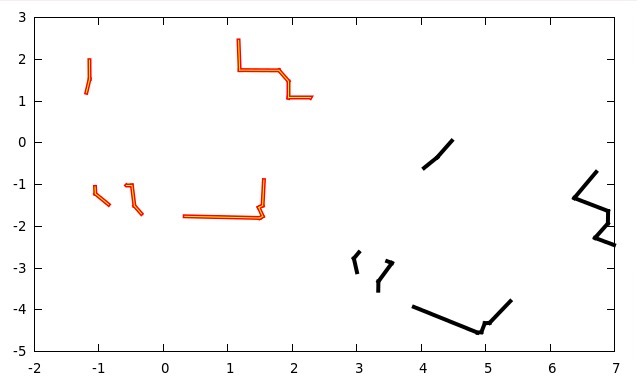
\includegraphics[width=1.0\textwidth]{images/foto_test/-5_-0.3_0.5236/plot.jpeg}
%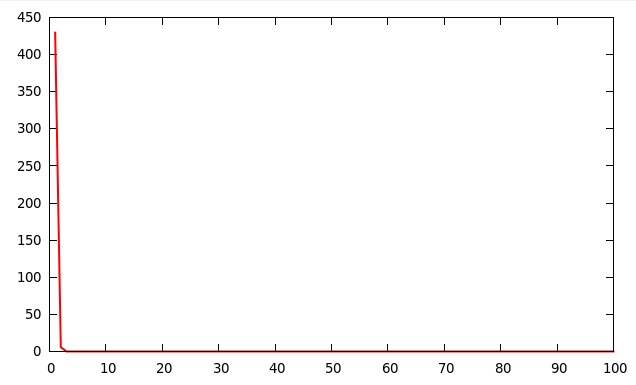
\includegraphics[width=1.0\textwidth]{images/foto_test/-5_-0.3_0.5236/chi.jpeg}
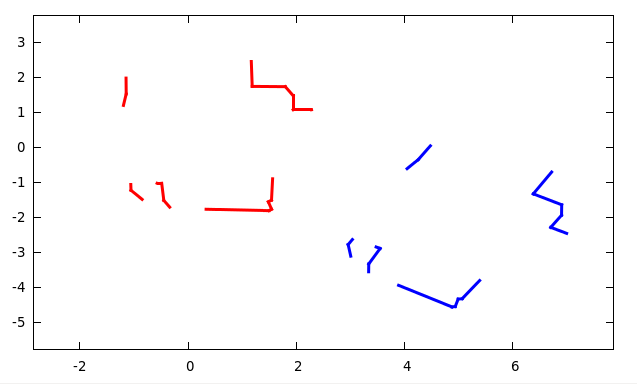
\includegraphics[width=0.9\textwidth]{images/foto_test/-5_-0.3_0.5236/before_after.png}
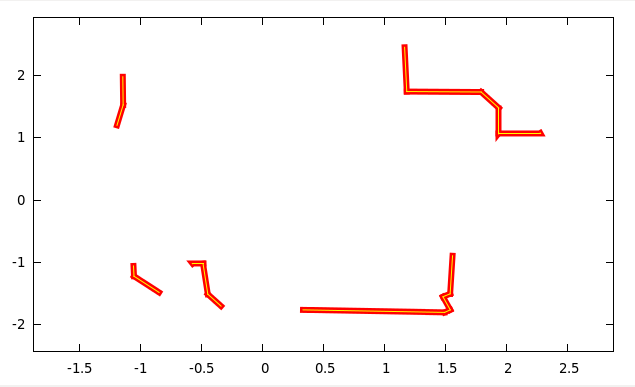
\includegraphics[width=0.9\textwidth]{images/foto_test/-5_-0.3_0.5236/result.png}
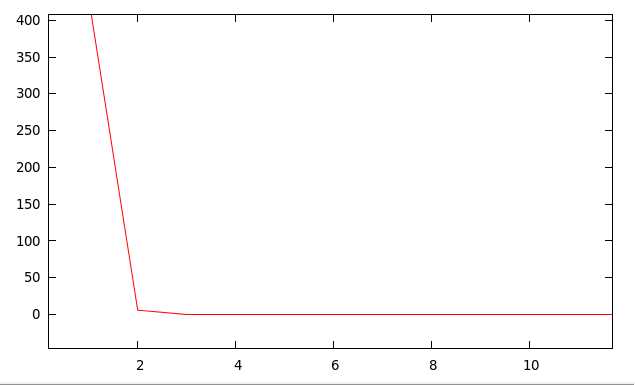
\includegraphics[width=0.9\textwidth]{images/foto_test/-5_-0.3_0.5236/chi_new.png}


\caption{LSE test 2}
\end{figure}

\begin{figure}[htbp]
\centering
%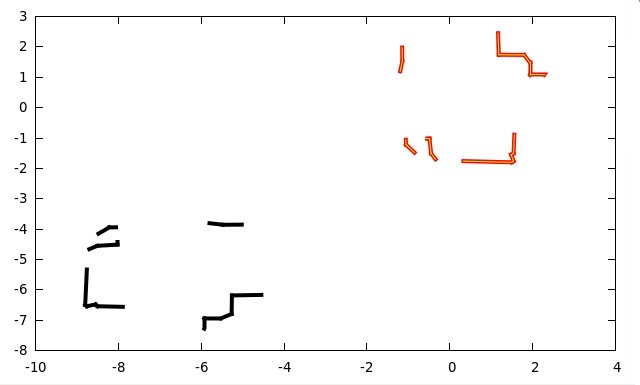
\includegraphics[width=1.0\textwidth]{images/foto_test/-5_7_-4.7124/plot.jpeg}
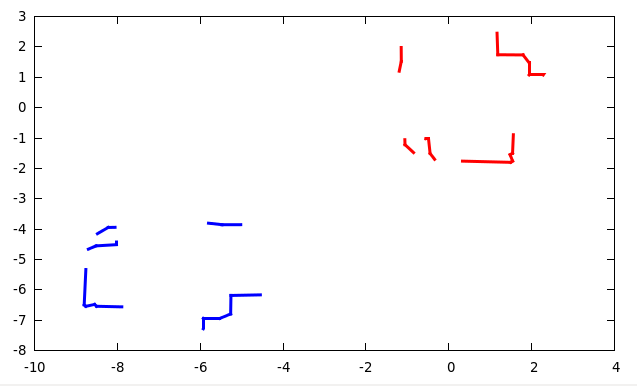
\includegraphics[width=0.9\textwidth]{images/foto_test/-5_7_-4.7124/before_after.png}
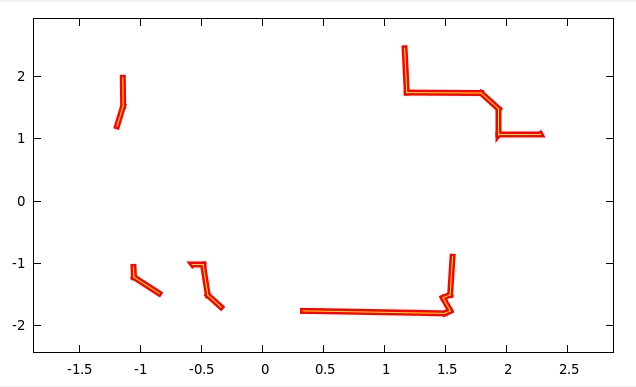
\includegraphics[width=0.9\textwidth]{images/foto_test/-5_7_-4.7124/result.png}
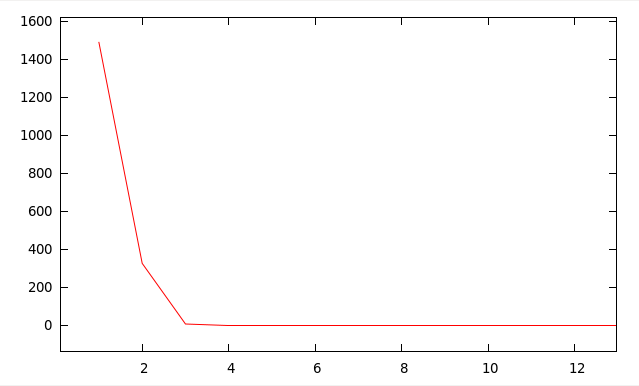
\includegraphics[width=0.9\textwidth]{images/foto_test/-5_7_-4.7124/chi_new.png}
\caption{LSE test 3}
\end{figure}

\begin{figure}[htbp]
\centering
%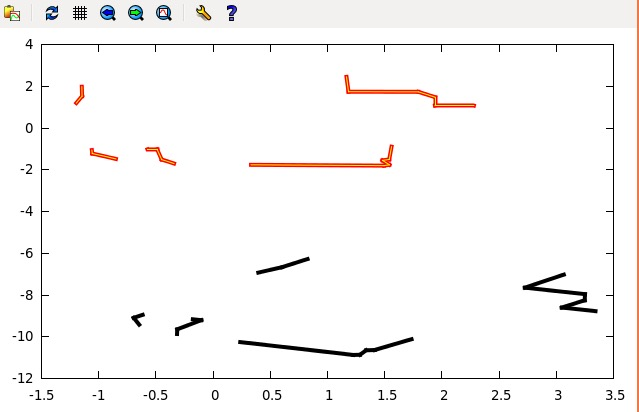
\includegraphics[width=1.0\textwidth]{images/foto_test/-5_7_0.5236/plot.jpeg}
%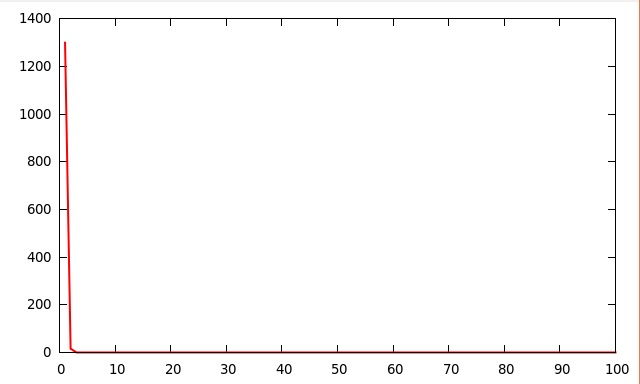
\includegraphics[width=1.0\textwidth]{images/foto_test/-5_7_0.5236/chi.jpeg}
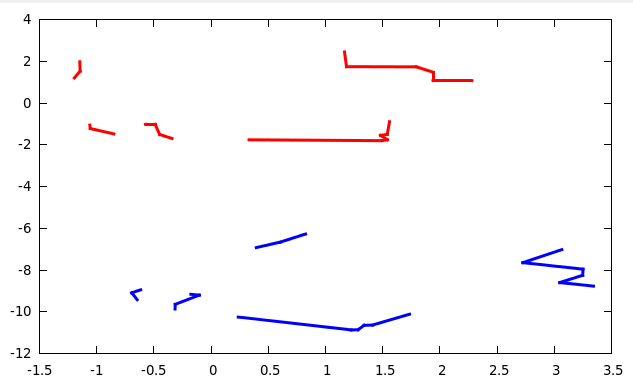
\includegraphics[width=0.9\textwidth]{images/foto_test/-5_7_0.5236/before_after.png}
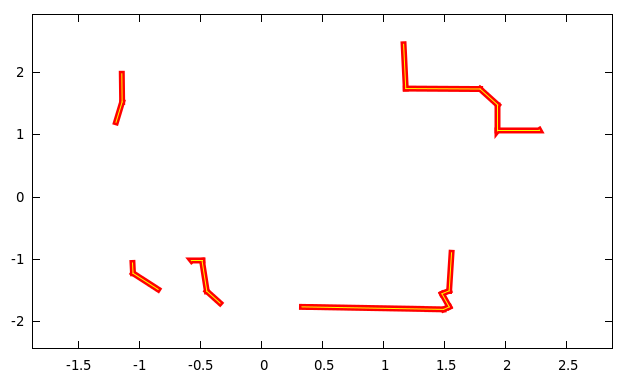
\includegraphics[width=0.9\textwidth]{images/foto_test/-5_7_0.5236/result.png}
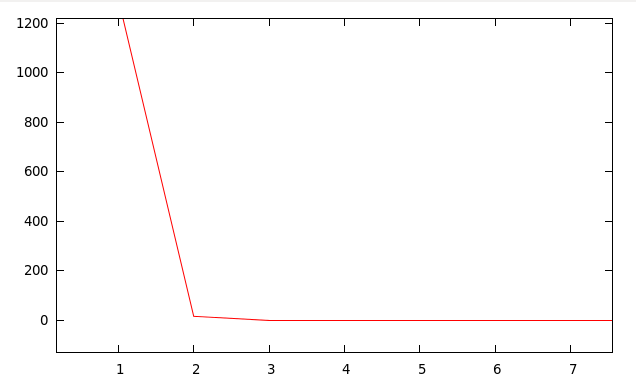
\includegraphics[width=0.9\textwidth]{images/foto_test/-5_7_0.5236/chi_new.png}

\caption{LSE test 4}
\end{figure}

\begin{figure}[htbp]
\centering
%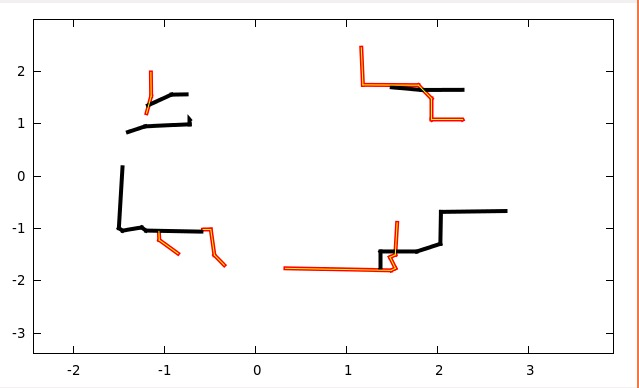
\includegraphics[width=1.0\textwidth]{images/foto_test/0.5_-0.3_-4.7124/plot.jpeg}
%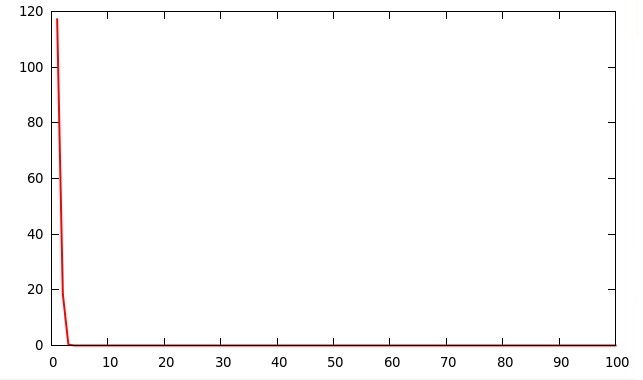
\includegraphics[width=1.0\textwidth]{images/foto_test/0.5_-0.3_-4.7124/chi.jpeg}
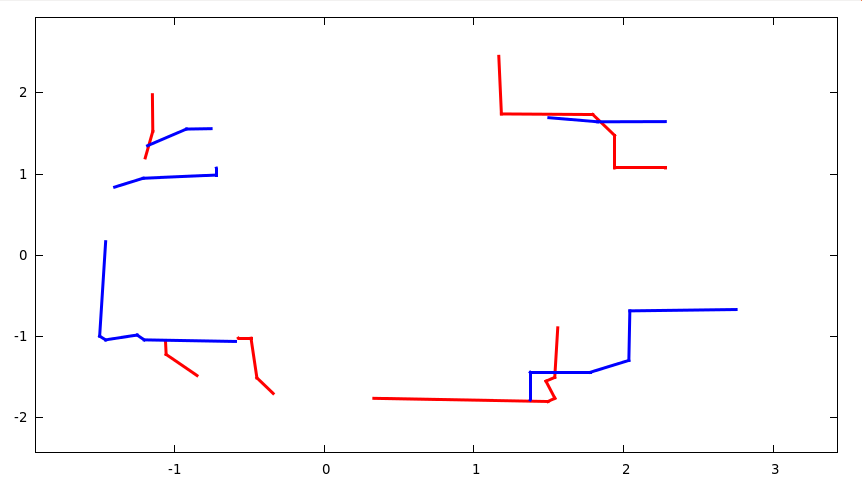
\includegraphics[width=0.9\textwidth]{images/foto_test/0.5_-0.3_-4.7124/before_after.png}
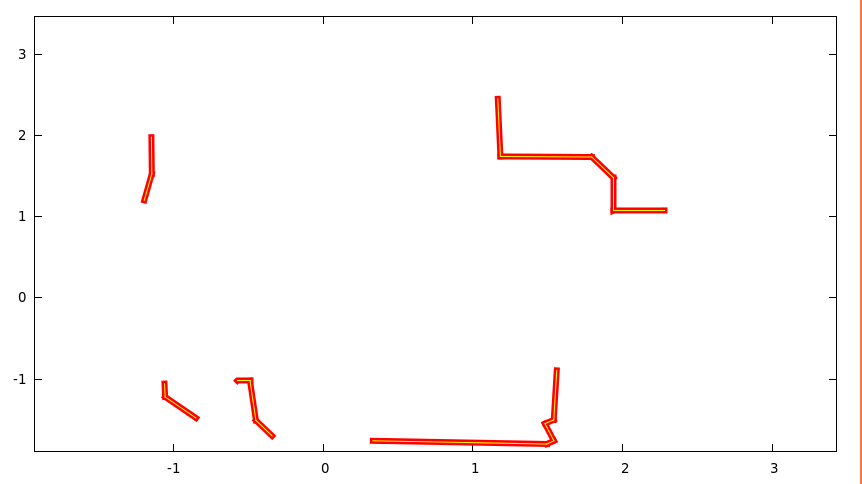
\includegraphics[width=0.9\textwidth]{images/foto_test/0.5_-0.3_-4.7124/result.png}
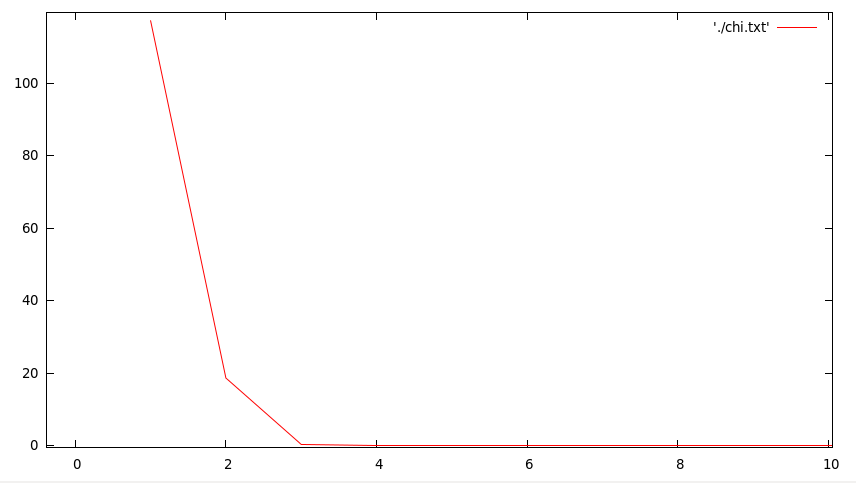
\includegraphics[width=0.9\textwidth]{images/foto_test/0.5_-0.3_-4.7124/chi_new.png}
\caption{LSE test 5}
\end{figure}

\begin{figure}[htbp]
\centering
%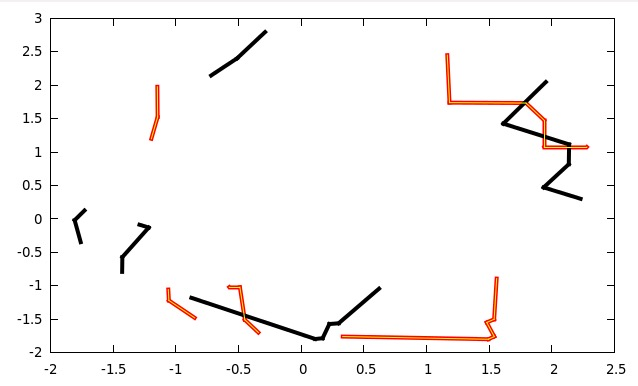
\includegraphics[width=1.0\textwidth]{images/foto_test/0.5_-0.3_0.5236/plot.jpeg}
%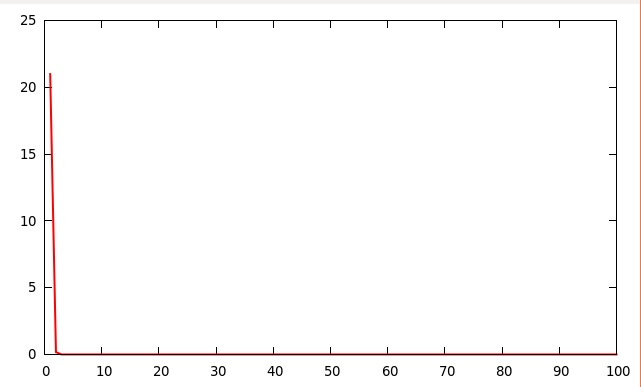
\includegraphics[width=1.0\textwidth]{images/foto_test/0.5_-0.3_0.5236/chi.jpeg}
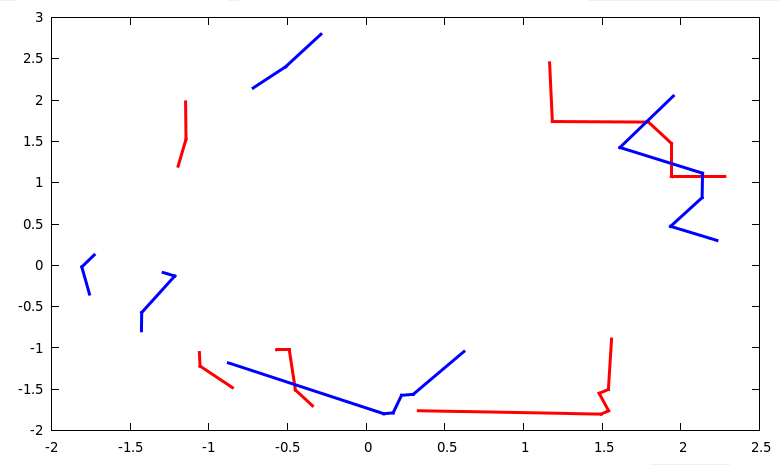
\includegraphics[width=0.9\textwidth]{images/foto_test/0.5_-0.3_0.5236/before_after.png}
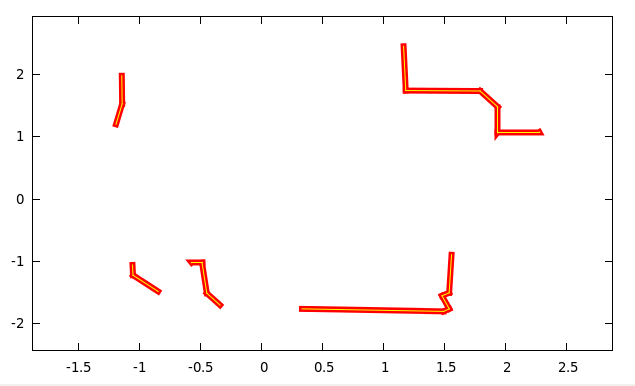
\includegraphics[width=0.9\textwidth]{images/foto_test/0.5_-0.3_0.5236/result.png}
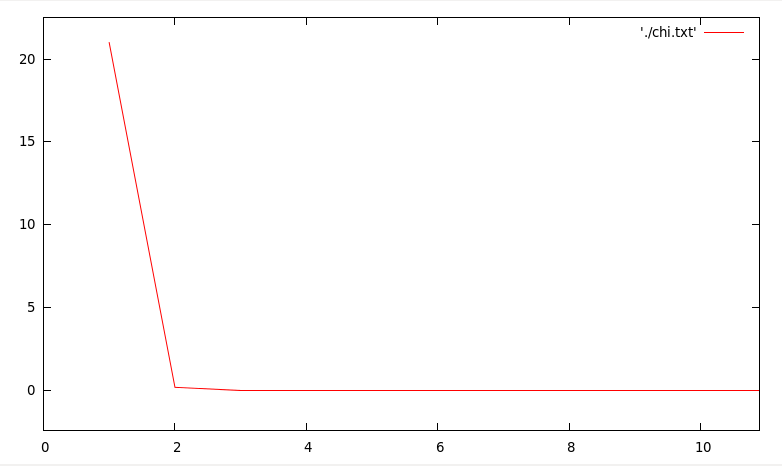
\includegraphics[width=0.9\textwidth]{images/foto_test/0.5_-0.3_0.5236/chi_new.png}
\caption{LSE test 6}
\end{figure}

\begin{figure}[htbp]
\centering
%\includegraphics[width=1.0\textwidth]{images/foto_test/0.5_7_-4.7124/plot.jpeg}
%\includegraphics[width=1.0\textwidth]{images/foto_test/0.5_7_-4.7124/chi.jpeg}
\includegraphics[width=0.9\textwidth]{images/foto_test/0.5_7_-4.7124/before_after.png}
\includegraphics[width=0.9\textwidth]{images/foto_test/0.5_7_-4.7124/result.png}
\includegraphics[width=0.9\textwidth]{images/foto_test/0.5_7_-4.7124/chi_new.png}
\caption{LSE test 7}
\end{figure}

\begin{figure}[htbp]
\centering
%\includegraphics[width=1.0\textwidth]{images/foto_test/0.5_7_0.5236/plot.jpeg}
%\includegraphics[width=1.0\textwidth]{images/foto_test/0.5_7_0.5236/chi.jpeg}
\includegraphics[width=0.9\textwidth]{images/foto_test/0.5_7_0.5236/before_after.png}
\includegraphics[width=0.9\textwidth]{images/foto_test/0.5_7_0.5236/result.png}
\includegraphics[width=0.9\textwidth]{images/foto_test/0.5_7_0.5236/chi_new.png}
\caption{LSE test 8}
\end{figure}

\subsection{Testing data association}
After verifying that simple tests executed in previous section gave good results, it was necessary to stress the system and prove its performance in a tougher case. Instead of creating a fictitious scan, whose extracted lines are obtained by applying an initial chosen transformation, let's consider two close robot poses $p_1$ and $p_2$, that differ in terms of odometric measurements. This means that, from these poses and scans acquired from them, we will certainly extract different lines or the same lines with different length and slope. \\ 
We asked LSE to compute the transformation $T_{21}$ that should map lines extracted in $p_2$'s reference frame to $p_1$'s. We then applied $T_{21}$ to $p_2$'s lines. The result is shown in Figure 5.15. As it is evident, LSE by itself is not able to furnish a good transformation to map correctly lines seen from $p_2$ to $p_1$'s reference frame, since even lines that are evidently the same are far from each other and differently rotated. 

So it is clear that LSE module needs to be integrated with some other sort of module to improve its performances; that is why, as shown in Figure 4.2, we coupled LSE with a data association module; the latter recalls iteratively LSE (which has an iterative nature of its own) correcting every time the set of initial couples with which LSE works. Such correction is made using last transformation $T_{21}$ returned by LSE at last iteration (at first launch of LSE it is possible to use an identity matrix). We move lines seen from $p_2$ to $p_1$'s frame and try to form couples of associations between the set of transformed lines and the ones in $p_1$'s frame. \\
As explained in 4.3.2, a first set of putative couples is formed by comparing the normals of lines candidate to be associated: if the dot product exceeds a given threshold, the two lines form a temporarily accepted couple. For our test, we used a threshold $NORM\_THRESHOLD = 0.8$.

A putative couple is kept in set to be returned if the distance between midpoints of involved lines is lesser than $MP\_THRESHOLD = 0.1^2$ and the difference between their slopes falls below $ANGLE\_THRESHOLD = \frac{5\pi}{180}$. \\
A shown in Figure 5.16, now the full system composed by LSE and data association is able to return a transformation $T_{21}$ that allows to optimally align $p_1$'s and $p_2$'s frames. In particular, Figure 5.17 shown the associations between lines obtained using the last $T_{21}$ returned. It is evident that even the data association process benefits of the coupling of the modules. By visual inspection, it can be noticed that the couple formed by LSE and data association manages to align two different frames, minimising the error during process.

\begin{figure}[htbp]
\centering
\includegraphics[width=1.0\textwidth]{images/two_frames/P_PTP_PT_after_LS.png}
\caption{The lines extracted from $p_1$(red), the ones extracted from $p_2$ (green) and the ones obtained after applying $T_{21}$ to lines in $p_2$ (blue)}
\end{figure}
\begin{figure}[htbp]
\centering
\includegraphics[width=1.0\textwidth]{images/two_frames/data_association_no_eval.png}
\caption{Lines acquired fron $p_1$	(red) and the ones seen from $p_2$ (green), after applying transformation $T_{21}$ returned by the couples of modules made by LSE and data association}
\end{figure}
\begin{figure}[htbp]
\centering
\includegraphics[width=1.0\textwidth]{images/two_frames/data_association.png}
\caption{Associations between lines seen from $p_1$ (red) and $p_2$'s transformed lines (green). Associations are shown in blue}
\end{figure}

A good question to answer is about a good number of iterations for data association module, i.e. how many times LSE module has to be called and how many times its output needs to be corrected. 
Recalling 5.4, at $j$-th execution of data association module, we obtain a global error measurement
\begin{equation}
	E_j = \frac{\chi_{j}}{a_j}
\end{equation}
where $a_j$ is the number of associations found at iteration $j$ and $\chi_{j}$ is the local error of LSE module at the $j$-th iteration of data association module. \\
Figure 5.18 shows that, after remaining constant up to 50th iteration, error $E_j$ almost falls down to zero and doesn't vary even after many other iterations. So, 50 proved to be a good choice when deciding how many times data association needs to be executed. 
\begin{figure}[htbp]
\centering
\includegraphics[width=1.0\textwidth]{images/chi.jpeg}
\caption{Number of iterations of data association module (X axis) and values of $E_j$ (Y axis)}
\end{figure}


\listoffigures
\listoftables
\end{document}